\documentclass[11pt]{article}
\usepackage[OT1]{fontenc}
\usepackage[utf8]{inputenc}
\usepackage[margin=1in]{geometry}
\usepackage{amsmath,amssymb,amsthm,mathtools}
\usepackage{enumitem,booktabs,array}
\usepackage{microtype}
\usepackage{xcolor}
\usepackage{tikz}
\usepackage{hyperref}
\usepackage[nameinlink,noabbrev]{cleveref}
\hypersetup{
  colorlinks=true,
  linkcolor=blue!45!black,
  citecolor=green!35!black,
  urlcolor=blue!55!black,
  pdftitle={A linear cycle-and-edge decomposition of every graph},
  pdfauthor={OpenAI}
}
\numberwithin{equation}{section}
\newtheorem{theorem}{Theorem}[section]
\newtheorem{lemma}[theorem]{Lemma}
\newtheorem{proposition}[theorem]{Proposition}
\newtheorem{corollary}[theorem]{Corollary}
\newtheorem{claim}[theorem]{Claim}
\theoremstyle{definition}
\newtheorem{definition}[theorem]{Definition}
\theoremstyle{remark}
\newtheorem{remark}[theorem]{Remark}
\newcommand{\abs}[1]{\left|#1\right|}
\newcommand{\ceil}[1]{\left\lceil#1\right\rceil}
\newcommand{\floor}[1]{\left\lfloor#1\right\rfloor}
\newcommand{\E}{\mathbb E}
\newcommand{\N}{\mathbb N}
\newcommand{\R}{\mathbb R}
\newcommand{\eps}{\varepsilon}
\setlist{itemsep=3pt,topsep=5pt}
\setlist[itemize]{label=\(\bullet\)}
\setlength{\emergencystretch}{2em}
\title{A linear cycle-and-edge decomposition of every graph}
\author{OpenAI}
\date{September 24, 2026}

\begin{document}
\maketitle

\begin{abstract}
We prove that every finite simple undirected graph on \(n\) vertices
has an edge partition into at most \(Cn\) simple cycles and single
edges, for an absolute constant \(C\). This resolves the
Erd\H{o}s--Gallai cycle decomposition conjecture positively.
\end{abstract}

\section{Introduction}\label{sec:introduction}

How efficiently can the edges of a graph be partitioned into cycles?
Single edges must also be allowed: a forest contains no cycle.
The Erd\H{o}s--Gallai cycle decomposition conjecture asserts that this
necessary allowance suffices for a universal linear bound.
Here and throughout, a cycle is simple and has length at least three.

\begin{theorem}\label{thm:main}
There is an absolute constant \(C>0\) such that, for every finite
simple undirected graph \(G\) with \(n\) vertices, \(E(G)\) has a
partition into at most \(Cn\) parts, each of which is the edge set of
a cycle or consists of a single edge.
\end{theorem}

The parts in this theorem may share vertices. They share no edges,
and every edge of \(G\) occurs in exactly one part. Isolated vertices
need not be covered, and the empty partition is permitted when
\(E(G)=\varnothing\).

The conjecture appears in the 1966 paper of Erd\H{o}s, Goodman and
P\'osa~\cite[Section~5]{EGP1966}, which explicitly distinguishes
unrestricted covers from edge-disjoint covers and records an
\(O(n\log n)\) upper bound. Conlon, Fox and
Sudakov~\cite{CFS2014} improved the general bound to
\(O(n\log\log n)\) in 2014. Buci\'c and
Montgomery~\cite{BM2024} subsequently proved the bound
\(O(n\log^*n)\); their paper appeared in journal form in 2024.
Here \(\log^*n\) is the number of logarithm iterations needed to
reach at most one. \Cref{thm:main} establishes the conjectured
linear bound. Its order is optimal, since a tree on \(n\) vertices
requires \(n-1\) single-edge parts. More sharply, complete bipartite
examples require \((3/2-o(1))n\) parts; see
\cite[Section~6]{BM2024} for this lower bound and its history.

Linear bounds were already known for important classes. Conlon, Fox
and Sudakov~\cite[Theorems~1.3 and~1.4]{CFS2014} proved them with high
probability for binomial random graphs, and deterministically for
graphs of linear minimum degree.
Kor\'andi, Krivelevich and Sudakov~\cite{KKS2015} obtained
asymptotically sharp counts over a broad range of random-graph
probabilities. For every fixed \(\alpha,\delta>0\), Gir\~ao,
Granet, K\"uhn and Osthus~\cite[Theorem~1.10(iii)]{GGKO2021}
proved that sufficiently large graphs of minimum degree at least
\(\alpha n\) admit at most \((3/2+\delta)n\) cycles and edges.
Akbari, Aloni, Beikmohammadi and Clow~\cite[Theorem~1.3]{AABC2025}
proved the bound \(n-1\) for graphs of positive order and maximum
degree at most four.
The general problem allows both sparse regions and vertices of
widely differing degrees.

The edge-disjoint requirement is essential to the problem. If cycles
and edges may overlap, Pyber~\cite{Pyber1985} proved that \(n-1\)
parts suffice to cover every graph of positive order. Akbari, Aloni,
Beikmohammadi and Clow~\cite[Theorem~1.7]{AABC2025} improved this
covering bound to \(n-2\) for graphs containing a cycle.
A cover of that kind does not supply a partition: deleting repeated
edges may break its cycles into many paths. Our construction keeps a
separate assignment for every original edge throughout.

\Cref{thm:main} also yields two cycle-only consequences. Here a graph is
\emph{Eulerian} if all its degrees are even; connectivity is not required.

\begin{corollary}\label{cor:eulerian-cycles}
Every finite simple undirected Eulerian graph on \(n\) vertices has an
edge partition into at most \(Cn\) cycles, with \(C\) from \Cref{thm:main}.

For every fixed \(\delta,p>0\), there exist \(\eps>0\) and an integer
\(n_0\ge1\) such that every finite simple undirected Eulerian graph \(G\)
on \(n\ge n_0\) vertices has an edge partition into at most
\(\Delta(G)/2+\delta n\) cycles, provided that every partition
\(V(G)=A\mathbin{\dot\cup}B\) with \(|A|,|B|\ge\eps n\) satisfies
\[
 e_G(A,B)\ge p|A||B|.
\]
Here \(\Delta(G)\) denotes the maximum degree, and \(e_G(A,B)\)
is the number of edges joining \(A\) to \(B\).
\end{corollary}

Any edge partition of \(G\) into cycles needs at least \(\Delta(G)/2\)
cycles, since a cycle uses at most two edges incident with a given
vertex. The second assertion attains this lower bound up to an
arbitrarily small linear error under the stated large-cut condition.

\begin{proof}
For the first claim, let the partition from \Cref{thm:main} have \(r\)
cycle parts and \(s\) single-edge parts, with \(r+s\le Cn\). The graph
formed by the latter edges has even degrees, since deleting cycles
preserves degree parity. Repeatedly removing a cycle preserves this
property and ends with no edges: every even graph with an edge contains
a cycle. This uses at most \(s\) cycles, for a total of at most
\(r+s\le Cn\). The equivalence of this \(O(n)\) Eulerian cycle bound
with the Erd\H{o}s--Gallai conjecture is recorded in
\cite[Section~1.1]{GGKO2021}.

The partition-cut condition in the second claim is exactly the
weakly-\((\eps,p)\)-quasirandom condition of
\cite[Section~1.2]{GGKO2021}. Their Proposition~6.3 proves that
Conjecture~1.14, the stated bound with these quantifiers, is equivalent
to their Erd\H{o}s--Gallai Conjecture~1.4, supplied by \Cref{thm:main}.
\end{proof}

Our argument builds on the expansion, hypergraph matching and
path-closing methods of Buci\'c and Montgomery~\cite{BM2024}, with
earlier reservoir and sparse-cut methods of Conlon, Fox and
Sudakov~\cite{CFS2014}.
We use Lov\'asz's path-and-cycle decomposition
theorem~\cite{Lovasz1968} and the Aharoni--Haxell matching
theorem~\cite{AH2000}, in the precise forms stated below.
The additional mechanism is an induction that saves vertices
across different scales while reserving enough edges to lift
cycles from the smaller graphs. A decomposition that repeatedly pays
a cost proportional to the full graph order can accumulate a factor
from the number of scales. Here the work over a suitable prefix is
charged to one expanding layer, and pair identifications save a fixed
fraction of that layer's order. The savings pay for the work outside
the recursive calls.

\subsection*{Outline of the proof}

All logarithms below are to base two. A graph has cut expansion
\(h\) when every cut has at least \(h\) times the size of its
smaller side in crossing edges.
We split the graph at successively smaller scales
\(D_j=n^{(0.95)^j}\). At scale \(D\), a small collection of long cycles
is removed, and the remaining edges are assigned to boxes of order at
most \(D^{1.02}\). Their vertex sets may overlap, but the total order
increases by only a factor \(1+O(1/\log D)\). Within each box, we
extract vertex-disjoint pieces with cut expansion \(D^{0.90}\).
Each residual box graph has average degree at most \(D^{0.95}\), so
the construction continues at the next scale.

Processing every expanding piece at every scale would accumulate too
much cost. Instead, we choose a layer whose total piece order pays
for an entire prefix, including a fixed number of further scales.
The pieces of this layer have two roles. First, an expanding graph
can be partitioned into linearly many completed parts and residual
graphs whose total order is an arbitrarily small fraction of its
own order (\Cref{lem:small-residue}). Second, part of its edge set
can be reserved for routing without destroying that conclusion.
The sparse graphs passed to the next scale retain their full box
vertex sets; the small-residue graphs produced when pieces are
processed are eventually handled by induction.

We describe the nonterminal case; the terminal cases are treated
separately in \Cref{sec:induction}. After the fixed gap in scales,
the unprocessed edges are sparse and
live on very small descendant boxes. We gather those boxes into
batches. Within each earlier box \(Y\), all but
\(O(\abs{Y}/\log D)\) vertices have small degree in the union of
that box's batch graphs. We pair these vertices in sufficiently large
intersections between a batch and a selected expanding piece, and
identify each pair. Edges between a folding set and vertices having
too many neighbors in that set are first partitioned into paths; reserved
routes close the trimmed remnants into cycles at linear cost. The
remaining graph can then be simplified after pair identification by
setting aside only linearly many edges as single-edge parts
(\Cref{lem:pair-folding,lem:batch-resolution}).

The quotient graphs have fewer vertices, so induction partitions
their edges into cycles and single edges. Each quotient edge retains
one original representative. At a paired vertex, the representatives
of a quotient cycle may enter through one member of the pair and leave
through the other. We join these two members by a path in the reserved
expanding piece. The routing lemma chooses these paths edge-disjointly,
with interiors that avoid the representative endpoints and are pairwise
disjoint within each cycle (\Cref{lem:routing}). Consequently each
quotient cycle lifts to one simple cycle. The degree bound is imposed
on the union of the batch graphs within each
earlier box, so the routing load does not grow with the number of batches.

In this case, write \(S\) for the total order of the selected layer.
All work outside the recursive calls costs \(O(S+n/\log D)\) parts.
The quotient orders sum to at most \(n-S/3+O(n/\log D)\), and the
small-residue graphs have total order at most \(S/100\). In the
resulting cost estimate, choosing \(C\) sufficiently large makes
the coefficient of \(S\) nonpositive. To absorb the remaining
\(O(Cn/\log D)\) overhead, we prove the stronger inductive bound
\(C\phi(n)n\), where
\[
 \phi(n)=\max\left\{\frac12,\,
                 1-\frac1{\sqrt{\log n}}\right\}
 \quad(n>1),\qquad \phi(1)=\frac12.
\]
The quotient graphs have order at most \(D^{0.30}\). Their smaller
value of \(\phi\) supplies a gain of order \(1/\sqrt{\log D}\),
which dominates the \(O(1/\log D)\) overlap cost.
All recursive graphs are strictly smaller, and all scale
requirements are fixed before the final constant \(C\) is chosen.

Section~\ref{sec:preliminaries} fixes the graph conventions and the two
external theorem inputs. Sections~\ref{sec:routing} and~\ref{sec:residue}
establish the routing
and small-residue tools. Section~\ref{sec:splitting} constructs the
scale layers, Section~\ref{sec:folding} combines folding with those
tools, and Section~\ref{sec:induction} completes the induction.

\section{Conventions and preliminary results}\label{sec:preliminaries}

\subsection{Graphs, partitions and scales}

Unless explicitly stated otherwise, graphs are finite, simple and
undirected. A path is simple and has at least one edge. The
\emph{order} of a graph is its number of vertices, including any
isolated vertices that have been retained. Temporary quotients
formed by identifying vertices may have loops or parallel edges;
these are removed before any decomposition theorem is applied.

An indexed family of subgraphs partitions a graph when their
assigned edge sets are pairwise disjoint and have the required
union. Each subgraph carries only its assigned edges, rather than
all edges induced by its vertex set. Different indices may have
overlapping, or even equal, vertex sets. Order sums count those
indices separately. Whenever edges from different members are
combined, we specify the assignment and account for the edges
that remain.

For disjoint vertex sets \(A,B\), write \(E_H(A,B)\) for the set
of edges of \(H\) between them and \(e_H(A,B)=|E_H(A,B)|\).
Write \(\partial_H U\) for
the edge boundary of \(U\subseteq V(H)\). An \(r\)-vertex graph
\(H\) has \emph{cut expansion at least \(h\)} if
\begin{equation}\label{eq:cut-expansion}
 |\partial_H U|\ge h\min\{|U|,r-|U|\}
 \qquad\text{for every }U\subseteq V(H).
\end{equation}
If \(r\ge2\), singleton cuts show that its minimum degree is at
least \(h\), and consequently \(r\ge h+1\).

All logarithms denoted by \(\log\) are to base two; \(\ln\)
denotes the natural logarithm. Scales \(D\) are real, and decimal
exponents denote exact rational numbers. Inequalities comparing
integer orders with real bounds have their literal meaning.
Asymptotic notation always refers to the scale tending to
infinity. Once the explicitly fixed parameters of a lemma have
been chosen, its implicit constants and lower scale threshold
are uniform over the graphs and orders allowed by that lemma.
In the final induction the finite list of parameters is fixed
first, a common lower cutoff \(D_*\) is fixed next, and only then
is \(C\) chosen.

\subsection{A path decomposition with controlled endpoints}

We use the following form of Lov\'asz's decomposition theorem.
Disjointness in its original statement means
edge-disjointness~\cite[Theorem~1]{Lovasz1968}; see also
\cite[Theorem~21]{BM2024}.

\begin{theorem}[Lov\'asz]\label{thm:lovasz}
The edges of a finite simple graph on \(n\) vertices can be
partitioned into at most \(\floor{n/2}\) paths and cycles.
\end{theorem}

The following consequence is recorded in
\cite[Corollary~22]{BM2024}. We include the deduction because
endpoint multiplicities are used in two different constructions.

\begin{corollary}\label{cor:endpoint-paths}
Every finite simple graph on \(n\) vertices has an edge
partition into paths such that each vertex is an endpoint of at
most two paths. In particular, the partition has at most \(n\)
paths.
\end{corollary}

\begin{proof}
For \(n=0\) there is nothing to prove. Otherwise add a vertex
\(v_0\) and join it to precisely the even-degree vertices of
the original graph, including the isolated vertices. Every old
vertex now has odd degree. In a path-and-cycle partition its
number of path-endpoint occurrences must therefore be odd and
positive.

Apply \Cref{thm:lovasz} to the augmented graph, and let \(p\)
be the number of path parts. The old vertices force \(2p\ge n\),
whereas the theorem gives
\[
 \ceil{n/2}\le p
 \le \text{number of parts}
 \le \floor{(n+1)/2}=\ceil{n/2}.
\]
Thus every part is a path. Each old vertex is an endpoint
exactly once: an old vertex with at least three endpoint
occurrences, together with the other old vertices, would force
at least \(n+2\) occurrences, although \(2p\le n+1\).

Delete \(v_0\) from these paths and discard any edgeless
remnants. Every old vertex is incident to at most one deleted
edge, so it gains at most one new endpoint occurrence. The
remaining paths partition the original edge set and have
endpoint load at most two. Each positive-length path contributes
two endpoint occurrences, proving the final count.
\end{proof}

\subsection{Disjoint representatives for hypergraphs}

A hypergraph here is a finite family of nonempty subsets of a
finite ground set. A matching is a subfamily of pairwise
disjoint edges. We use the following sufficient condition,
from the hypergraph Hall theorem of Aharoni and
Haxell~\cite{AH2000}, in the bounded-rank form stated in
\cite[Theorem~6]{BM2024}.

\begin{theorem}[Aharoni--Haxell]\label{thm:aharoni-haxell}
Let \(s\) be a positive integer and let
\((\mathcal H_i)_{i\in J}\) be a finite indexed family of
hypergraphs on a common ground set. Suppose every edge is
nonempty and has size at most \(s\). If, for every nonempty
\(I\subseteq J\), the union
\(\bigcup_{i\in I}\mathcal H_i\) has a matching of size
strictly greater than \(s(|I|-1)\), then there are edges
\(E_i\in\mathcal H_i\), one for each \(i\in J\), that are
pairwise disjoint.
\end{theorem}

One may pass from the uniform-size version to this statement
by padding each edge occurrence with private fresh vertices.
Every matching before padding remains a matching after padding,
and disjoint representatives after padding have disjoint
original projections. The hypergraphs need not be distinct, and equal
edges in different indexed hypergraphs cause no difficulty.

\subsection{Elementary probabilistic estimates}

We use linearity of expectation, Markov's inequality, the union
bound, and the following binomial estimates. They are stated
explicitly to fix constants for the sampling arguments.

\begin{lemma}\label{lem:chernoff}
If \(X\) is binomial with mean \(\mu\), then
\[
 \Pr(X\le\mu/2)\le e^{-\mu/8},
 \qquad
 \Pr(X\ge2\mu)\le e^{-\mu/3}.
\]
\end{lemma}

\begin{proof}
For \(X\) a sum of independent Bernoulli variables,
\(\E e^{tX}\le\exp(\mu(e^t-1))\).
Apply Markov's inequality with \(t=-\ln2\) for the lower
tail and \(t=\ln2\) for the upper tail. The resulting exponents
are \(-\mu(1-\ln2)/2\) and \(-\mu(2\ln2-1)\),
respectively. They are at most \(-\mu/8\) and \(-\mu/3\).
\end{proof}

\section{Routing with team constraints}
\label{sec:routing}

A demand specifies two distinct vertices to be joined.  Demands are indexed,
so several demands may specify the same pair.  Besides edge-disjointness of
all routes, we will need internal vertex-disjointness for specified groups
of routes.  The following lemma supplies both requirements.  Its proof uses
the hypergraph formulation and expansion-to-connectivity method of
Buci\'c and Montgomery~\cite[Proposition~8 and Lemma~9]{BM2024}.
The vertex tokens introduced in the proof impose a separate
internal-disjointness constraint for each team; different teams
compete only for graph edges.

\begin{lemma}[Routing]\label{lem:routing}
Let $P$ be a graph of order $r\ge 2$ with cut expansion $h>0$, and put
\begin{equation}\label{eq:routing-radii}
  g=\ceil{8(r/h)\log(2r)},\qquad
  \ell=2g\bigl(1+\ceil{\log r}\bigr).
\end{equation}
Let $\mathcal D$ be a finite set of demands, where demand $p$ has distinct
endvertices $x_p,y_p\in V(P)$.  Suppose that each vertex occurs as an
endvertex in at most $k$ demands, where $k\ge 1$.  Partition $\mathcal D$
into teams of size at most $b$, where $b\ge 1$, and give each demand a set
$Z_p\subseteq V(P)$ of at most $z$ vertices, where $z\ge 0$.
If
\begin{equation}\label{eq:routing-condition}
  h\ge 64\bigl(\ell^2(k+b)+z\bigr),
\end{equation}
then there are simple $x_p$--$y_p$ paths $Q_p$ in $P$, one for each
$p\in\mathcal D$, with the following properties:
\begin{enumerate}[label=\textup{(\roman*)}]
  \item each $Q_p$ has length at most $\ell$ and no internal vertex in $Z_p$;
  \item the paths $Q_p$ are pairwise edge-disjoint;
  \item the internal vertex sets of paths in the same team are pairwise
    disjoint.
\end{enumerate}
The sets $Z_p$ may contain $x_p$ or $y_p$: their restrictions concern only
internal vertices.  If a route must also avoid another demand's endvertices
internally, those vertices may be included in its set $Z_p$.
\end{lemma}

\begin{proof}
There is nothing to prove when $\mathcal D$ is empty.  Suppose it is
nonempty, and write $c(p)$ for the team of demand $p$.

\paragraph{A hypergraph obstruction.}
Take a resource set that is the tagged disjoint union of $E(P)$ and the
tokens $(v,c)$, where $v\in V(P)$ and $c$ is a team.  For each demand $p$,
form a hypergraph $\mathcal H_p$ on this resource set.  Its hyperedges
correspond to all simple $x_p$--$y_p$ paths of length at most $\ell$ whose
internal vertices avoid $Z_p$.  A candidate path contributes its graph
edges and the token $(v,c(p))$ for each of its internal vertices.  A path
of length $t\ge 1$ therefore contributes $2t-1\le 2\ell$ resources.
In particular all hyperedges are nonempty, and all the hypergraphs are
finite.  A choice of pairwise disjoint representatives from the
$\mathcal H_p$ gives exactly the three required properties.

We verify the sufficient condition of \Cref{thm:aharoni-haxell} with
$s=2\ell$.  Suppose, for a contradiction, that it fails for a nonempty
$I\subseteq\mathcal D$.  Let $\mathcal M$ be a maximum matching in
$\bigcup_{p\in I}\mathcal H_p$.  Then
$\abs{\mathcal M}\le 2\ell(\abs I-1)$.  Let $F\subseteq E(P)$ be the
graph-edge resources used by $\mathcal M$, and put
\[
  Y_c=\{v\in V(P):(v,c)\text{ is used by }\mathcal M\}.
\]
Each matching member uses at most $\ell$ graph edges and at most $\ell$
tokens, so
\begin{equation}\label{eq:routing-obstruction-budgets}
  \abs F\le 2\ell^2\abs I,\qquad
  \sum_c\abs{Y_c}\le 2\ell^2\abs I.
\end{equation}
These estimates allow several matching members to come from one demand;
no restriction on their demand indices is being imposed.

For each team let $m_c=\abs{\{p\in I:c(p)=c\}}\le b$.  Thus
\[
  \sum_{p\in I}\abs{Y_{c(p)}}
  =\sum_c m_c\abs{Y_c}
  \le 2b\ell^2\abs I.
\]
Consequently the set
$I_1=\{p\in I:\abs{Y_{c(p)}}\le 4b\ell^2\}$ has size at least
$\abs I/2$.  Choose an inclusion-maximal set $I_2\subseteq I_1$ whose
endpoint pairs are pairwise vertex-disjoint.  Every demand in $I_1$ meets
one of these selected pairs.  The two vertices of any selected pair
occur in at most $2k$ demands in total, so
\begin{equation}\label{eq:routing-pair-count}
  \abs{I_2}\ge\frac{\abs{I_1}}{2k}
  \ge\frac{\abs I}{4k}.
\end{equation}
We will also use the global endpoint count
\begin{equation}\label{eq:routing-endpoint-count}
  2\abs I\le kr.
\end{equation}

\paragraph{A small ball for each selected demand.}
For $p\in I_2$, define
\[
  W_p=(Z_p\cup Y_{c(p)})\setminus\{x_p,y_p\},\qquad
  P_p=(P-F)-W_p.
\]
Here the first deletion removes edges and the second removes vertices.
Both endpoints remain in $P_p$.  By \eqref{eq:routing-condition},
\begin{equation}\label{eq:routing-forbidden-budget}
  \abs{W_p}\le z+4b\ell^2
  \le 4\bigl(z+(k+b)\ell^2\bigr)
  \le h/16\le h/4.
\end{equation}
Set $T=\ell/2=g(1+\ceil{\log r})$, an integer.  If the balls of
radius $T$ about both $x_p$ and $y_p$ in $P_p$ had size greater than
$r/2$, they would intersect.  Joining their paths to an intersection
vertex gives an $x_p$--$y_p$ walk of length at most $2T=\ell$; deleting
closed subwalks gives a simple path of no greater length.  It uses no
edge of $F$ and no vertex of $W_p$.  Its internal vertices are also
different from $x_p,y_p$, and hence avoid both $Z_p$ and $Y_{c(p)}$.
Its hyperedge in $\mathcal H_p$ is therefore disjoint from $\mathcal M$,
contrary to maximality of that matching.

For every $p\in I_2$ we may consequently choose an endpoint $s_p$ whose
radius-$T$ ball in $P_p$ has size at most $r/2$.  Let
$S=\{s_p:p\in I_2\}$.  These roots are distinct because the selected
endpoint pairs are disjoint.  Each root retains its demand label: write
$p(s)$ for the unique $p\in I_2$ with $s=s_p$.  In particular,
\begin{equation}\label{eq:routing-small-root-balls}
  \abs{\{v:\operatorname{dist}_{P_{p(s)}}(s,v)\le T\}}\le r/2
  \qquad(s\in S).
\end{equation}

\paragraph{Growth with different forbidden sets.}
The deleted-edge budget may be too large to grow a ball from one root.
We first grow unions of balls, retaining each root's graph, and then
alternate halving the root set with further growth until one root remains.
For a nonempty $A\subseteq S$ and an integer $t\ge 0$, put
\[
  B_t(A)=\bigcup_{s\in A}
  \{v\in V(P_{p(s)}):\operatorname{dist}_{P_{p(s)}}(s,v)\le t\}.
\]
These are unions of balls in their respective graphs; the forbidden set
is kept with its root throughout.  We claim that
\begin{equation}\label{eq:routing-union-growth}
  \abs{B_{t+1}(A)}
  \ge\left(1+\frac{h}{2r}\right)\abs{B_t(A)}
\end{equation}
whenever
\begin{equation}\label{eq:routing-growth-threshold}
  0<\abs{B_t(A)}\le r/2,
  \qquad \abs F\le h\abs{B_t(A)}/4.
\end{equation}

To prove this, let $B=B_t(A)$ and assign to each $v\in B$ one root
$s(v)\in A$ that reaches $v$ within $t$ steps in $P_{p(s(v))}$.
Consider a boundary edge $vw$ of $B$, with $v\in B$ and $w\notin B$.
It extends this particular root's path whenever $vw\notin F$ and
$w\notin W_{p(s(v))}$.  In that event $w\in B_{t+1}(A)\setminus B$.
Because $P$ is simple, at most $\abs{W_{p(s(v))}}\le h/4$ boundary
edges at $v$ fail the latter condition.  Cut expansion and
\eqref{eq:routing-growth-threshold} therefore leave at least
\[
  h\abs B-(h/4)\abs B-\abs F\ge(h/2)\abs B
\]
usable boundary edges.  Each new vertex receives at most $r$ such
edges.  Thus at least $h\abs B/(2r)$ new vertices are reached, proving
\eqref{eq:routing-union-growth}.

It follows that, for every integer $t\ge 0$,
\begin{equation}\label{eq:routing-growth-block}
  \abs{B_t(A)}\ge 1\ \text{ and }\quad
  \abs F\le h\abs{B_t(A)}/4
  \quad\Longrightarrow\quad
  \abs{B_{t+g}(A)}>r/2.
\end{equation}
Indeed, the conclusion is immediate by monotonicity if the starting
union already has size greater than $r/2$.  Otherwise, if it still had
size at most $r/2$ after $g$ more steps, all intervening unions would
have size at most $r/2$, while their monotonicity would preserve the
edge-deletion threshold.  We could apply
\eqref{eq:routing-union-growth} at all $g$ steps.  Singleton cuts in
the simple graph $P$ give $0<h\le r-1<r$, and the elementary inequality
$\log(1+h/(2r))\ge h/(4r)$ then yields
\[
  \abs{B_{t+g}(A)}
  \ge \left(1+\frac{h}{2r}\right)^g\abs{B_t(A)}
  \ge 2^{gh/(4r)}
  \ge (2r)^2>r/2,
\]
a contradiction.  This also verifies the growth time with the ceiling
in the definition of $g$.

\paragraph{Restarting after halving the roots.}
Initially $B_0(S)=S$.  By \eqref{eq:routing-obstruction-budgets},
\eqref{eq:routing-pair-count}, and \eqref{eq:routing-condition},
\[
  \abs F\le 2\ell^2\abs I
  \le 8k\ell^2\abs S\le h\abs S/4.
\]
The growth block \eqref{eq:routing-growth-block} gives
$\abs{B_g(S)}>r/2$.

Suppose now that a nonempty root set $A$ has
$\abs{B_t(A)}>r/2$ and $\abs A\ge 2$.  Partition $A$ into two
nonempty sets whose sizes differ by at most one.  Their radius-$t$
ball unions together cover $B_t(A)$, so one of them, say $A'$, satisfies
\[
  \abs{A'}\le\ceil{\abs A/2},\qquad
  \abs{B_t(A')}>r/4.
\]
The original matching has a bound independent of the number of retained
roots: by \eqref{eq:routing-obstruction-budgets},
\eqref{eq:routing-endpoint-count}, and \eqref{eq:routing-condition},
\begin{equation}\label{eq:routing-restart-budget}
  \abs F\le 2\ell^2\abs I
  \le \ell^2kr\le hr/64
  < h\abs{B_t(A')}/4.
\end{equation}
Thus another growth block gives $\abs{B_{t+g}(A')}>r/2$.

Start with $A=S$ at radius $g$ and repeat this operation until only one
root remains.  After $j$ halvings the number of roots is at most
$\ceil{\abs S/2^j}$; this follows inductively from rounding each half
upward.  Hence at most $\ceil{\log\abs S}$ halvings are needed,
including zero if $\abs S=1$.  At termination a single root has a ball
larger than $r/2$ at an integer radius at most
\[
  g\bigl(1+\ceil{\log\abs S}\bigr)
  \le g\bigl(1+\ceil{\log r}\bigr)=T.
\]
This contradicts \eqref{eq:routing-small-root-balls} and monotonicity of
that root's balls.

There is therefore no set $I$ for which the matching condition fails.
Applying \Cref{thm:aharoni-haxell} gives disjoint hypergraph
representatives, and their paths prove the lemma.
\end{proof}

For later estimates, the exact radii also give the useful uniform bound
\begin{equation}\label{eq:routing-length-bound}
  \ell\le 108(r/h)(\log r)^2
  =O\bigl((r/h)(\log r)^2\bigr).
\end{equation}
Indeed, $h<r$ and $r\ge 2$ imply
$g\le 9(r/h)\log(2r)$,
$\log(2r)\le 2\log r$, and
$1+\ceil{\log r}\le 3\log r$.

\section{Expansion in small reservoirs}\label{sec:residue}

We next process a graph containing a spanning expanding subgraph.
Reserving vertices and edges to connect and close paths is already
central to the cycle decomposition argument of Conlon, Fox and
Sudakov~\cite[Section~3]{CFS2014}. Our aim here is to leave residual
graphs with arbitrarily small total vertex order, so that their
recursive cost can be paid by the later folding savings. At a scale $D$, put
\[
  \sigma=D^{0.90},\qquad \tau=D^{0.74}.
\]
Throughout this section the order $r$ lies in
$\sigma\le r\le D^{1.02}$.  All assertions for sufficiently large $D$
are uniform over the graphs and orders in this range.  Their thresholds
may depend on the fixed positive constants in the statements.

\subsection{Splitting the expanding edges}

\begin{lemma}[Edge splitting]\label{lem:edge-split}
Fix $c>0$ and a positive integer $l$.  For all sufficiently large $D$,
if an $r$-vertex graph $P$ has cut expansion at least
$h_0\ge cD^{0.90}$ and $D^{0.90}\le r\le D^{1.02}$, then its edge set
can be partitioned into $l$ spanning subgraphs, each with cut expansion
at least $h_0/(2l)$.
\end{lemma}

\begin{proof}
Assign each edge independently and uniformly to one of $l$ classes.
Fix a cut whose smaller side has size $u\ge1$, and let $e$ be its
number of edges in $P$.  In any fixed class its size is binomial with
mean $e/l\ge h_0u/l$.  By \Cref{lem:chernoff}, the probability that
this class has fewer than $h_0u/(2l)$ cut edges is at most
\[
  \exp\bigl(-h_0u/(8l)\bigr).
\]
There are at most $2\binom ru\le2r^u$ choices of a cut with smaller
side of size $u$.  Thus the probability of any failure is at most
\[
  2l\sum_{u=1}^{\floor{r/2}}
       \bigl(r\exp(-h_0/(8l))\bigr)^u=o(1).
\]
Indeed, $h_0\ge cD^{0.90}$ while $\log r\le1.02\log D$, so the base
of this geometric sum tends to zero uniformly.  A successful
assignment gives the required edge partition.  Each class is taken on
the full vertex set of $P$.
\end{proof}

\subsection{Expansion after vertex sampling}

The issue is to control every sampled cut without a union bound over
all vertex subsets. Buci\'c and Montgomery establish connectivity by
short paths through a random vertex set, using successive exposures
and well-expanding subsets~\cite[Section~4]{BM2024}. In the polynomial cut-expansion
range used here, we instead fix a small family of neighborhood unions
and show that it approximates every possible failing sampled cut.

\begin{lemma}[Vertex sampling]\label{lem:vertex-sampling}
Fix $c'>0$ and $p\in(0,1)$.  Let $P$ have order
$D^{0.90}\le r\le D^{1.02}$ and cut expansion at least
$h=c'D^{0.90}$.  Select each vertex independently with probability $p$
to form $V'$.  With probability $1-o(1)$ as $D\to\infty$, all of the
following hold:
\begin{equation}\label{eq:residue-sampling-properties}
\begin{gathered}
  |V'|\le2pr,\qquad
  |N_P(v)\cap V'|\ge ph/2\quad(v\in V(P)),\\
  P[V']\text{ has cut expansion at least }\tau=D^{0.74}.
\end{gathered}
\end{equation}
The error term is uniform over the stated graphs and orders, with
$c'$ and $p$ fixed.
\end{lemma}

\begin{proof}
The minimum degree of $P$ is at least $h$.  The order bound and all
the sampled-degree bounds fail with total probability at most
\begin{equation}\label{eq:residue-size-degree-error}
  \exp(-pr/3)+r\exp(-ph/8)=o(1)
\end{equation}
by \Cref{lem:chernoff}.  We prove the expansion assertion by first
controlling a deterministic family of cuts and then approximating
any hypothetical failing sampled cut by a member of that family.

\paragraph{A deterministic witness family.}
In a failing sampled cut, the sampled-degree bound forces most vertices
on the smaller side to have many neighbors on that side. A small
selection from that side can hit their neighborhoods while exposing few
vertices across the cut; this is why we enumerate unions of a small
number of original neighborhoods.
Set
\[
  M=C_p\log r,\qquad C_p=16/p,\qquad
  s=\ceil{4rM/h}.
\]
For sufficiently large $D$, we have $M/h<1$ and $s\le r$.
Before sampling $V'$, form the family
\[
  \mathcal U=
  \left\{\ \bigcup_{v\in S}N_P(v):
                   S\subseteq V(P),\ |S|\le s\ \right\}.
\]
Its members are unions of open neighborhoods in the original graph,
and its size satisfies
\begin{equation}\label{eq:residue-witness-count}
  |\mathcal U|
  \le\sum_{t=0}^s\binom rt
  \le(s+1)r^s
  =\exp\!\bigl(O((1+rM/h)\log r)\bigr).
\end{equation}
Repeated neighborhood unions only decrease this count.

We claim that, with probability $1-o(1)$, simultaneously for every
$U\in\mathcal U$ satisfying
$\min\{|U|,r-|U|\}\ge ph/8$, one has
\begin{equation}\label{eq:residue-witness-cut}
  e_P(U\cap V',V'\setminus U)
     \ge\frac{p^2}{4}|\partial_P U|.
\end{equation}
Fix such a $U$, and put $e=|\partial_P U|$.  Expansion gives
$e\ge ph^2/8$.  Partition its cut edges into at most $2r$ matchings:
greedily color the cut edges, observing that an edge has fewer than
$2r$ other edges incident with its endpoints.  Fix one such coloring
for each cut before sampling.  The matching classes of size less than
$e/(4r)$ contain fewer than $e/2$ edges in total.  In a remaining
matching of size $m$, the indicators that both endpoints of an edge
belong to $V'$ are independent, since its edges have disjoint
endpoints.  Its retained size is therefore binomial with mean $p^2m$.
The probability of retaining fewer than $p^2m/2$ edges is at most
\[
  \exp(-p^2m/8)
  \le\exp\bigl(-p^2e/(32r)\bigr)
  \le\exp\bigl(-p^3h^2/(256r)\bigr).
\]
When none of these matching events fails, the large classes retain
at least $(p^2/2)(e/2)=p^2e/4$ edges.  Independence between different
matching classes or between different cuts is unnecessary: a union
bound bounds the probability of any failure of
\eqref{eq:residue-witness-cut} by
\begin{equation}\label{eq:residue-witness-error}
  2r|\mathcal U|\exp\bigl(-p^3h^2/(256r)\bigr)=o(1).
\end{equation}
To verify this uniformly, the scale restrictions give
\[
  \frac{h^2}{r}\ge(c')^2D^{0.78},\qquad
  \frac rh\le(c')^{-1}D^{0.12},\qquad
  M=O_p(\log D).
\]
Consequently the positive term in the exponent coming from
\eqref{eq:residue-witness-count} is
$O_{p,c'}(D^{0.12}(\log D)^2)$, while the negative term in
\eqref{eq:residue-witness-error} has magnitude at least a fixed
positive multiple of $D^{0.78}$.

\paragraph{Approximating a failing cut.}
Fix an outcome satisfying the size and degree bounds and all of
\eqref{eq:residue-witness-cut}.  Suppose, for a contradiction, that
some $A\subseteq V'$ satisfies
\begin{equation}\label{eq:residue-bad-cut}
  0<a=|A|\le |V'|/2,
  \qquad e_P(A,V'\setminus A)<\tau a.
\end{equation}
We may assume $D$ is large enough that $\tau<ph/4$.  If $a\le ph/4$,
every vertex of $A$ has more than $ph/4$ neighbors in $V'\setminus A$,
because its sampled degree is at least $ph/2$ and it has at most
$a-1$ neighbors in $A$.  This contradicts
\eqref{eq:residue-bad-cut}.  Thus
\begin{equation}\label{eq:residue-bad-cut-size}
  a>ph/4.
\end{equation}
Let
\[
  A_{\mathrm{good}}=
    \{v\in A:|N_P(v)\cap A|\ge ph/4\}.
\]
Each vertex in $A\setminus A_{\mathrm{good}}$ has more than $ph/4$
neighbors across the sampled cut.  Hence
\begin{equation}\label{eq:residue-exceptional-vertices}
  |A\setminus A_{\mathrm{good}}|
       \le\frac{4\tau a}{ph}.
\end{equation}

We now make a separate auxiliary random choice solely to prove the
existence of a suitable set $S\subseteq A$.  Include each vertex of
$A$ independently with probability $q=M/h$.  For every
$v\in A_{\mathrm{good}}$, the probability that $S$ misses all its
neighbors in $A$ is at most
\[
  (1-q)^{ph/4}\le\exp(-pM/4).
\]
Thus the probability of any required miss is at most
$r\exp(-pM/4)\le r^{-3}<1/4$.  Here the chosen value of $C_p$
is more than sufficient, since all logarithms are base two.
Also $\E|S|=aM/h$.  If $T(S)$ denotes the number of vertices of
$V'\setminus A$ with a neighbor in $S$, then a union bound for each
such vertex gives
\[
  \E T(S)
  \le\frac Mh\sum_{v\in V'\setminus A}|N_P(v)\cap A|
  =\frac Mh e_P(A,V'\setminus A)
  <\frac{\tau Ma}{h}.
\]
Markov's inequality shows that each of the events
$|S|>4aM/h$ and $T(S)>4\tau Ma/h$ has probability at most $1/4$.
The sum of these three failure probabilities is less than one.
We can therefore choose $S$ satisfying all three desired properties:
\begin{equation}\label{eq:residue-hitting-set}
\begin{gathered}
  |S|\le4aM/h,\qquad T(S)\le4\tau Ma/h,\\
  S\cap N_P(v)\ne\varnothing
      \quad(v\in A_{\mathrm{good}}).
\end{gathered}
\end{equation}
The auxiliary choice is made after $V'$ and $A$ have been fixed; the
uniform event \eqref{eq:residue-witness-cut} was already established
for every possible resulting neighborhood union.

Put $U=\bigcup_{v\in S}N_P(v)$.  Since
$|S|\le4aM/h\le4rM/h$, we have $U\in\mathcal U$.  The vertices of
$A$ absent from $U$ are all exceptional in
\eqref{eq:residue-exceptional-vertices}, and the vertices of
$U\cap V'$ outside $A$ are counted by $T(S)$.  Consequently
\begin{equation}\label{eq:residue-cut-approximation}
  \delta:=|(U\cap V')\mathbin{\triangle}A|
   \le\frac{4\tau a}{ph}+\frac{4\tau Ma}{h}
   =O_p\!\left(\frac{\tau Ma}{h}\right)=o(a).
\end{equation}
In the last step we used
$\tau M/h=O_{p,c'}(D^{-0.16}\log D)=o(1)$.
Both sides of the cut in the \emph{original} graph are large:
\[
  |U|\ge |A|-\delta=a-\delta,
  \qquad
  r-|U|\ge |V'\setminus U|
           \ge |V'\setminus A|-\delta\ge a-\delta.
\]
For sufficiently large $D$, these are at least $a/2>ph/8$.
Applying \eqref{eq:residue-witness-cut} and the expansion of $P$
therefore gives
\begin{equation}\label{eq:residue-approximating-cut-lower}
  e_P(U\cap V',V'\setminus U)\ge \frac{p^2ha}{8}.
\end{equation}
On the other hand, changing the side of one vertex changes the size
of a cut in a simple $r$-vertex graph by at most $r-1$.  Changing
the $\delta$ vertices in \eqref{eq:residue-cut-approximation} yields
\[
  e_P(U\cap V',V'\setminus U)
       \le e_P(A,V'\setminus A)+r\delta
       <\tau a+r\delta.
\]
The ratio of this upper bound to $ha$ is at most
\begin{equation}\label{eq:residue-cut-perturbation}
  \frac\tau h+
       O_p\!\left(\frac{\tau Mr}{h^2}\right)
  =O_{p,c'}(D^{-0.16})+
       O_{p,c'}(D^{-0.04}\log D)=o(1),
\end{equation}
contradicting \eqref{eq:residue-approximating-cut-lower}.
Thus no cut \eqref{eq:residue-bad-cut} exists.  Together with
\eqref{eq:residue-size-degree-error} and
\eqref{eq:residue-witness-error}, this proves the lemma.

All uses of $o(1)$ above occur after $p$ and $c'$ have been fixed.
In particular, an arbitrarily small fixed positive sampling
probability changes the cutoff but does not change any of the
strict exponent inequalities.
\end{proof}

\subsection{Closing paths through three reservoirs}

Buci\'c and Montgomery use three vertex classes and reserved connecting
subgraphs to close paths through a class avoided by the original
path~\cite[Section~2.2 and Lemma~23]{BM2024}. We use three disjoint reservoirs of
arbitrarily small fixed relative order. Every edge has both endpoints
outside at least one of them. After reserving the connecting edges,
we can therefore assign each remaining edge to such a complement,
partition that graph into paths, and close the paths through its
reservoir. The preceding sampling lemma supplies the internal expansion
needed for these routes. Unused reserved edges between a reservoir and
its complement are taken singly, leaving only unused reserved edges
inside reservoirs for recursion.

\begin{lemma}[Small residue]\label{lem:small-residue}
Fix $\eta>0$ and $c>0$.  For all sufficiently large $D$, let $G$ be
an $r$-vertex graph with
$D^{0.90}\le r\le D^{1.02}$ containing a spanning subgraph of cut
expansion at least $cD^{0.90}$.  Then $E(G)$ has a partition into at
most $9r$ completed parts, each a simple cycle or a single edge,
and the edge sets of at most three residual simple graphs.  The
residual graphs have pairwise disjoint vertex sets contained in
$V(G)$, their total order is at most $\eta r$, and each has order
strictly less than $r$.
\end{lemma}

\begin{proof}
Write $c_0=\min\{c,1\}$, and fix
\[
  p=\min\{\eta/12,1/12\},\qquad
  h=(c_0/6)\sigma.
\]
In particular, $3p<1$, $6p\le\eta$, and $2p<1$.
By \Cref{lem:edge-split}, the edges of the given spanning expanding
subgraph can be partitioned into three spanning subgraphs
$P_1,P_2,P_3$, each of cut expansion at least $h$.

\paragraph{Disjoint reservoirs and bounded representative loads.}
Label the vertices independently, using each label $i\in\{1,2,3\}$
with probability $p$ and a fourth label with probability $1-3p$.
Let $V_i$ be the vertices with label $i$.  These three sets are
pairwise disjoint, and each marginal $V_i$ is a Bernoulli-$p$
sample for the fixed graph $P_i$.  By \Cref{lem:vertex-sampling}
and a union bound over the three marginal failure probabilities,
we can choose the labels so that, for each $i$,
\begin{equation}\label{eq:residue-three-reservoirs}
\begin{gathered}
  |V_i|\le2pr,\qquad
  |N_{P_i}(v)\cap V_i|\ge ph/2\quad(v\in V(G)),\\
  P_i[V_i]\text{ has cut expansion at least }\tau.
\end{gathered}
\end{equation}
Independence between these three success events is not required.
The neighbor assertion makes $V_i$ nonempty and gives every vertex
of $V_i$ a neighbor in $V_i$, so $|V_i|\ge2$.

For each $i$, reserve all edges
$E_i^{\mathrm{in}}=E(P_i[V_i])$.  Also reserve two edges from each
$v\in V(G)\setminus V_i$ to two distinct representatives in $V_i$.
The representatives can be chosen so that at most
\begin{equation}\label{eq:residue-representative-capacity}
  k_0=\ceil{8r/(ph)}
\end{equation}
of these edges are incident with any one vertex of $V_i$.
Indeed, process the two choices for every outside vertex in turn.
At any point fewer than $2r$ edges have been chosen, so the number
of representatives already at capacity $k_0$ is at most
$2r/k_0\le ph/4$.  There are at least $ph/2$ potential
representatives for the next choice by
\eqref{eq:residue-three-reservoirs}.  Excluding the saturated ones
and, for the second choice at a vertex, its first representative,
leaves at least $ph/4-1>0$ choices for sufficiently large $D$.
This greedy procedure proves the claim.  Denote the selected
outside-to-representative edges by $E_i^{\mathrm{out}}$.

For a fixed $i$, the internal and outside reservations are disjoint.
Reservations for different values of $i$ also have disjoint edge
sets, because they belong to the edge-disjoint graphs $P_i$.
Let
\[
  E_{\mathrm{res}}=
     \bigcup_{i=1}^3(E_i^{\mathrm{in}}\cup E_i^{\mathrm{out}})
\]
be the entire reserved edge set.

\paragraph{The complementary path partitions.}
Every edge in $E(G)\setminus E_{\mathrm{res}}$ has both endpoints
outside at least one $V_i$, since its two endpoints meet at most two
of the three disjoint reservoirs.  Assign each such edge to one
such index $i$, choosing just one index if several are available.
This gives edge-disjoint graphs $G_i$ on $V(G)\setminus V_i$ whose
edge sets partition all nonreserved edges.
By \Cref{cor:endpoint-paths}, each $G_i$ has a partition into
positive-length simple paths, with each vertex an endpoint at most
twice.  Since each path has two endpoint occurrences, its path
family $\mathcal P_i$ has size at most $|V(G)\setminus V_i|\le r$.
An empty edge set contributes no paths.

For each endpoint occurrence of $v$ in $\mathcal P_i$, assign one
of its two reserved edges in $E_i^{\mathrm{out}}$, using different
edges for different occurrences.  This is possible by the endpoint
load bound.  For a path $Q\in\mathcal P_i$ with distinct endpoints
$x,y$, let $x',y'\in V_i$ be their assigned representatives.
When $x'\ne y'$, issue one demand between them in $P_i[V_i]$.
When $x'=y'$, no routing demand is necessary.
Every demand-end occurrence uses a different reserved edge at its
representative.  Hence the total demand load at each vertex of
$V_i$ is at most $k_0$.

\paragraph{Routing and simple cycles.}
Apply \Cref{lem:routing} separately in each $P_i[V_i]$, with
expansion parameter $\tau$, endpoint load $k=k_0$, singleton teams
($b=1$), and no forbidden vertices ($z=0$).  We check its numerical
hypothesis using the actual order $r_i=|V_i|$.  This graph has order
at least two and cut expansion at least $\tau$, and therefore
$\tau\le r_i-1$.  The value $\ell_i$ in \Cref{lem:routing} satisfies
\[
  \ell_i=O\!\left(\frac r\tau(\log r)^2\right),
  \qquad k_0=O_{p,c}\!\left(\frac rh\right).
\]
Here the ceiling in \eqref{eq:residue-representative-capacity}
is absorbed because $r/h\ge6$.  Consequently
\begin{equation}\label{eq:residue-routing-margin}
\begin{aligned}
  \ell_i^2(k_0+1)
   &=O_{p,c}\!\left(
        \frac{r^3}{\tau^2h}(\log r)^4\right)\\
   &=O_{p,c}(D^{0.68}(\log D)^4)
     =o(D^{0.74})=o(\tau).
\end{aligned}
\end{equation}
Thus \eqref{eq:routing-condition} holds for all sufficiently large
$D$.  The lemma supplies pairwise edge-disjoint simple routing
paths for all the distinct-representative demands in this reservoir.
All their edges are in the reserved set $E_i^{\mathrm{in}}$.

For $Q$ as above with $x'\ne y'$, join its endpoints by the edge
$xx'$, the routing path from $x'$ to $y'$, and the edge $y'y$.
Every new internal vertex lies in $V_i$, while $Q$ is entirely
outside $V_i$.  The resulting closed walk is therefore a simple
cycle.  When $x'=y'$, the two reserved edges themselves form a
simple two-edge connection from $x$ to $y$ through that
representative, and again close $Q$ to a simple cycle.  Its two
reserved edges are distinct because $x\ne y$.  In this case even a
one-edge path $Q$ produces a triangle; with different
representatives the resulting cycle has at least four edges.
Thus every completed cycle has length at least three.

The cycles are edge-disjoint.  Their original path edges partition
the nonreserved edges; each assigned representative edge is used
once; and the routing paths are edge-disjoint within each $P_i[V_i]$.
These three types of edges are disjoint by reservation.  The
reservations in different $P_i$ are also edge-disjoint, regardless
of vertex overlaps among different cycles.

\paragraph{Counting and the exact remaining edge sets.}
We have produced at most
$\sum_i|\mathcal P_i|\le3r$ cycles.  Take every unused edge in
$\bigcup_iE_i^{\mathrm{out}}$ as a single-edge part, using at most
\[
  \sum_{i=1}^3 2|V(G)\setminus V_i|\le6r
\]
further parts.  The number of completed parts is therefore at most
$9r$.

For each $i$, let $H_i$ be the graph on $V_i$ consisting of exactly
the unused edges of $E_i^{\mathrm{in}}$.  These are the only
remaining edges: every nonreserved edge was placed in a path,
every reserved outside edge was used in a cycle or taken singly,
and every reserved internal edge was used by a routing path or
placed in $H_i$.  In particular, $H_i$ is not defined by taking
all remaining edges of the original induced graph $G[V_i]$;
nonreserved edges, including ones with both endpoints in a
reservoir, were already assigned to the appropriate complementary
graphs.  This accounts for every original edge exactly once.

The graphs $H_i$ are simple, have the pairwise disjoint vertex sets
$V_i$, and satisfy
\begin{equation}\label{eq:residue-final-order}
  \sum_{i=1}^3|V(H_i)|
     =\sum_{i=1}^3|V_i|\le6pr\le\eta r,
  \qquad |V(H_i)|\le2pr\le r/6<r.
\end{equation}
Isolated vertices may be retained; a residual graph with no edges
may alternatively be omitted.  The only parameters fixed before
increasing $D$ were $\eta,c$ and the constants determined from
them.  This completes the proof.
\end{proof}

\section{Splitting at a scale}
\label{sec:splitting}

The first operation below splits the graph into small boxes, allowing a
small amount of vertex overlap.  The second operation extracts expanding
pieces on disjoint vertex sets within each box.  Only edges leave when a
piece is extracted: the residual graph retains every box vertex.  Thus
every earlier piece vertex still occurs in a descendant box when the
operations are iterated.  The overlapping split
and its inverse-logarithmic order potential adapt the expander
splitting argument of Buci\'c and Montgomery~\cite[Lemma~14]{BM2024}.
Here we stop at a prescribed scale and obtain a total box order
of \(N(1+O(1/\log D))\), which will be charged in the final induction.

\begin{lemma}[Splitting at a scale]\label{lem:scale-split}
There are absolute constants $D_{\mathrm{sp}}$ and $C_0$ such that, for
every real $D\ge D_{\mathrm{sp}}$, every graph $G$ on a nonempty vertex
set of order $N$ and with average degree at most $D$ admits the following
two successive operations.  One may take $C_0=2$.
\begin{enumerate}[label=\textup{(\roman*)}]
\item\label{item:scale-boxes}
Remove a family $\mathcal C$ of edge-disjoint cycles, each of length at
least $D^{1.01}$, where
\begin{equation}\label{eq:scale-cycle-cost}
  \abs{\mathcal C}\le \frac{N}{2D^{0.01}}.
\end{equation}
Partition the remaining edges into graphs $G_Y$ on an indexed family
$\mathcal Y$ of vertex sets, called boxes.  These satisfy
\begin{equation}\label{eq:scale-box-order}
\begin{gathered}
  \bigcup_{Y\in\mathcal Y}Y=V(G),\qquad
  1\le \abs Y\le D^{1.02},\\
  \sum_{Y\in\mathcal Y}\abs Y
    \le \left(1+\frac{C_0}{\log D}\right)N.
\end{gathered}
\end{equation}
The graphs $G_Y$ contain only their assigned edges; their vertex sets
may overlap.

\item\label{item:scale-expanders}
Put $\sigma=D^{0.90}$.  For each box $Y$, partition $E(G_Y)$ into
the edge sets of a family $\mathcal R_Y$ of graphs $R$ and a graph $H_Y$.
The vertex sets of the graphs in $\mathcal R_Y$ are pairwise disjoint
subsets of $Y$.  Each $R$ has cut expansion at least $\sigma$ and order
\begin{equation}\label{eq:scale-piece-order}
  \sigma\le \abs{V(R)}\le D^{1.02}.
\end{equation}
The residual graph $H_Y$ is taken on all of $Y$, including isolated
vertices, and satisfies
\begin{equation}\label{eq:scale-residual-degree}
  \frac{2\abs{E(H_Y)}}{\abs Y}\le D^{0.95}.
\end{equation}
\end{enumerate}
Thus the cycles in $\mathcal C$, the pieces $R$, and the residual graphs
$H_Y$ together partition $E(G)$.
\end{lemma}

We first give the elementary long-cycle argument used to find the
overlapping splits. It is the depth-first-search and bypass argument
of Buci\'c and Montgomery~\cite[Lemma~25]{BM2024}, with constants
suited to the present scale cutoff. Related depth-first-search balance
arguments appear in Ben-Eliezer, Krivelevich and
Sudakov~\cite[Lemma~2.3]{BKS2012}; Krivelevich~\cite[Theorem~1]{Krivelevich2019}
gives a stronger general criterion for long cycles from local expansion.
For a vertex set $U$ in a graph $H$, write
$N_H(U)=\bigcup_{v\in U}N_H(v)$; its external neighbor set is
$N_H(U)\setminus U$.

\begin{lemma}[Vertex expansion gives a long cycle]
\label{lem:split-vertex-expansion}
Fix $\eps=1/32$.  For every sufficiently large integer $u$, put
$\alpha=\eps/\log^2 u$.  If a graph $H$ of order $u$ satisfies
\begin{equation}\label{eq:split-vertex-expansion}
  \abs{N_H(U)\setminus U}\ge\alpha\abs U
  \qquad\left(0<\abs U\le\frac u2\right),
\end{equation}
then $H$ contains a simple cycle of length greater than
\begin{equation}\label{eq:split-long-cycle-length}
  q(u)=\frac{\alpha^2u}{100}
      =\frac{\eps^2u}{100\log^4u}.
\end{equation}
\end{lemma}

\begin{proof}
The expansion condition implies that $H$ is connected: in a
disconnected graph some component has order between $1$ and $u/2$ and
has no external neighbors.

Run a depth first search.  Its state consists of the unexplored
vertices, a stack whose vertices in stack order form a simple path, and the finished
vertices.  Initially the stack consists of one vertex, all other
vertices are unexplored, and none are finished.  If the top vertex of
the stack has an unexplored neighbor, push such a neighbor onto the
stack.  Otherwise pop the top vertex and mark it finished.  At all
times there are no edges between finished and unexplored vertices:
when a vertex is finished it has no unexplored neighbor, and the
unexplored set subsequently only shrinks.  Connectivity ensures that
the stack cannot become empty while an unexplored vertex remains, so
this search finishes all vertices.

The number of unexplored vertices minus the number of finished
vertices starts at $u-1$, ends at $-u$, and decreases by exactly one at
every push or pop.  Consequently there is a state at which these two
numbers are exactly equal, say to $t$.  Let $P$ be the stack path at
that state, and let $L=\abs{V(P)}=u-2t$.  If $t\ge u/3$, then
$0<t\le u/2$, and all external neighbors of the unexplored set lie on
$P$.  Applying \eqref{eq:split-vertex-expansion} gives
$L\ge\alpha t\ge\alpha u/3$.  If $t<u/3$, then
$L>u/3\ge\alpha u/3$, since $\alpha\le1$ for the values of $u$ under
consideration.  Thus in either case
\begin{equation}\label{eq:split-stack-order}
  L\ge\frac{\alpha u}{3}.
\end{equation}

Write $q=q(u)$ and $j=\floor q$.  We may assume $q\ge1$, since
$u/\log^4u$ tends to infinity.  In particular $j\ge1$, and
\[
  j+1\le2q=\frac{\alpha^2u}{50}
       \le\frac{\alpha u}{6}\le\frac L2.
\]
Partition $P$ into three consecutive vertex segments $X,J,Z$, with
$\abs J=j$, distributing the other $L-j$ vertices as evenly as
possible between $X$ and $Z$.  Both outer segments have order at least
\[
  \floor{\frac{L-j}{2}}
    \ge\frac{L-j-1}{2}\ge\frac L4.
\]
These inequalities include the integer rounding needed to make the
three segments nonempty.

Suppose first that $H-J$ has a path from $X$ to $Z$.  Choose one of
minimum length among all such paths, with endpoints $x\in X$ and
$z\in Z$.  A shortest path is simple.  Its interior contains no vertex
of $X$ or $Z$, because encountering either set internally would give a
shorter path between the two sets.  It also avoids $J$.  Since
$X,J,Z$ partition $V(P)$, the chosen path meets $P$ only at $x,z$.
Its union with the $x$--$z$ subpath of $P$ is therefore a simple cycle.
That subpath contains all $j$ vertices of $J$ and has at least $j+1$
edges; the new path has at least one edge.  The cycle consequently has
at least $j+2\ge3$ edges, and its length is greater than $q$.

It remains to show that such a path must exist.  Otherwise $X$ and
$Z$, each connected by its segment of $P$, lie in distinct components
of $H-J$.  Separate the component containing $X$ from the union of all
other components, which contains $Z$, and let $A$ be the smaller of
these two sets.  Then
\[
  \frac L4\le\abs A\le\frac{u-j}{2}\le\frac u2,
  \qquad N_H(A)\setminus A\subseteq J.
\]
Expansion and \eqref{eq:split-stack-order} imply
\[
  j\ge\alpha\abs A\ge\frac{\alpha L}{4}
    \ge\frac{\alpha^2u}{12}
    >\frac{\alpha^2u}{100}=q,
\]
contrary to $j=\floor q$.  This proves the lemma.
\end{proof}

\begin{proof}[Proof of \Cref{lem:scale-split}]
We prove the two operations in order.  All lower bounds imposed on $D$
in this proof are absolute and hold simultaneously for every
$D\ge D_{\mathrm{sp}}$ after one choice of $D_{\mathrm{sp}}$.

\paragraph{Removing long cycles.}
Choose a maximal family $\mathcal C$ of edge-disjoint cycles in $G$
whose lengths are at least $D^{1.01}$.  Since
$\abs{E(G)}\le ND/2$, we have
\[
  \abs{\mathcal C}D^{1.01}\le\abs{E(G)}\le\frac{ND}{2},
\]
which proves \eqref{eq:scale-cycle-cost}.  Integral cycle lengths are
compared with the real threshold as stated, equivalently with
$\ceil{D^{1.01}}$.  Delete these cycle edges and retain the entire
vertex set.  By maximality the remaining graph has no cycle of length
at least $D^{1.01}$.  Every graph subsequently formed in the first
operation is a subgraph of this remainder, so it inherits this
prohibition.

\paragraph{A sparse external neighborhood.}
Put $T=D^{1.02}$ and $\eps=1/32$.  We claim that every current graph
$H$ of order $u>T$ has a nonempty vertex set $U$ such that
\begin{equation}\label{eq:split-sparse-neighborhood}
  \abs U\le\frac u2,\qquad
  \abs{N_H(U)\setminus U}
    <\frac{\eps\abs U}{\log^2u}.
\end{equation}
Otherwise \Cref{lem:split-vertex-expansion} supplies a cycle longer
than $q(u)$ as defined in \eqref{eq:split-long-cycle-length}.
To obtain a contradiction uniformly for every $u>T$, including $u$
arbitrarily large relative to $D$, observe that $x/\log^4x$ is
increasing for $\ln x>4$, as follows by differentiating.  Moreover,
\begin{equation}\label{eq:split-uniform-margin}
  \frac{q(T)}{D^{1.01}}
    =\frac{\eps^2}{100(1.02)^4}
       \frac{D^{0.01}}{(\log D)^4}
    \longrightarrow\infty\qquad(D\longrightarrow\infty).
\end{equation}
Choose $D_{\mathrm{sp}}$ large enough that $T$ is in the range of
\Cref{lem:split-vertex-expansion}, that $T>e^4$, and that
$q(T)>D^{1.01}$.  Then $q(u)>D^{1.01}$ for every $u>T$,
contradicting the inherited cycle prohibition.  This proves
\eqref{eq:split-sparse-neighborhood}.

\paragraph{The overlapping split and its edge assignment.}
For such a set $U$, put $B=N_H(U)\setminus U$ and form two children
on vertex sets
\[
  V_1=U\cup B,\qquad V_2=V(H)\setminus U.
\]
Assign to the first child every edge of $H$ with both endpoints in
$V_1$, and assign to the second child every other edge of $H$.
Every edge incident with $U$ has both endpoints in $U\cup B$.
Consequently every edge assigned to the second child has both endpoints
in $V_2$.  This is an edge partition into two simple subgraphs; in
particular, edges with both endpoints in the overlap $B$ are assigned
only to the first child.  The child vertex sets cover the parent and
have intersection exactly $B$.  All vertices of each specified child
set are retained, even when isolated in its assigned graph.

Writing $s=\abs U$, $b=\abs B$, $u_1=s+b$ and $u_2=u-s$, we have
$1\le s\le u/2$ and $b<\eps s/\log^2u$.  For sufficiently large
$D$, therefore,
\begin{equation}\label{eq:split-child-orders}
\begin{gathered}
  1\le u_1\le\frac{3u}{4},\qquad 1\le u_2<u,\\
  u_1+u_2=u+b
      \le u+\frac{\eps u_1}{\log^2u}.
\end{gathered}
\end{equation}
Indeed $\eps/\log^2u\le1/2$ gives
$u_1<(3/2)s\le3u/4$, and $u_2<u$ follows from $s\ge1$.
Repeat this split whenever the current order exceeds $T$.
Both child orders are positive integers strictly smaller than their
parent order, so the resulting binary splitting tree is finite.
Its leaves give the graphs $G_Y$ on boxes of order at most $T$.
The child cover property gives $\bigcup_Y Y=V(G)$, and the edge
assignments at each split show that the leaf graphs partition exactly
the edges left after the cycle removal.

\paragraph{Controlling the sum of box orders.}
The sum of child orders can exceed the parent order by $b$.  The
following potential pays for this overlap.  For every real $x\ge1$
define
\begin{equation}\label{eq:split-potential}
  f(x)=1+\frac1{\log(T/2)}
         -\frac1{\log(\max\{x,T/2\})}.
\end{equation}
For $T\ge4$, this is nondecreasing and
\begin{equation}\label{eq:split-potential-range}
  1\le f(x)\le1+\frac1{\log(T/2)}\le2.
\end{equation}
At a split of a graph of order $u>T$, put
$M=\max\{u_1,T/2\}$.  By \eqref{eq:split-child-orders} and $u>T$,
we have $M\le3u/4$.  Both logarithms below are positive, and
\begin{equation}\label{eq:split-potential-decrement}
\begin{aligned}
  f(u)-f(u_1)
    &=\frac1{\log M}-\frac1{\log u}\\
    &=\frac{\log(u/M)}{\log M\,\log u}
      \ge\frac{\log(4/3)}{\log^2u}.
\end{aligned}
\end{equation}
Monotonicity also gives $f(u_2)\le f(u)$.  Hence, using
\eqref{eq:split-child-orders},
\begin{equation}\label{eq:split-potential-subadditivity}
\begin{aligned}
  u_1f(u_1)+u_2f(u_2)
    &\le (u_1+u_2)f(u)
         -\frac{u_1\log(4/3)}{\log^2u}\\
    &\le uf(u)
         +\frac{u_1}{\log^2u}
                 \bigl(\eps f(u)-\log(4/3)\bigr)\\
    &\le uf(u).
\end{aligned}
\end{equation}
For the last step, \eqref{eq:split-potential-range} gives
$\eps f(u)\le1/16<\log(4/3)$.  Repeatedly applying
\eqref{eq:split-potential-subadditivity} in the finite splitting tree,
and using $f\ge1$ on its leaves, proves
\[
  \sum_{Y\in\mathcal Y}\abs Y
    \le\sum_{Y\in\mathcal Y}\abs Y f(\abs Y)
    \le Nf(N)
    \le N\left(1+\frac1{\log(T/2)}\right).
\]
This argument also applies if $N\le T$, when the tree has just its
root.  Since $T=D^{1.02}$ and $D\ge4$,
\[
  \frac1{\log(T/2)}
    =\frac1{1.02\log D-1}\le\frac2{\log D}.
\]
This proves \eqref{eq:scale-box-order} with $C_0=2$ and finishes
operation~\ref{item:scale-boxes}.

\paragraph{Extracting pieces of cut expansion $\sigma$.}
This repeated removal of sparse cuts follows the small-side charging
method used by Conlon, Fox and Sudakov~\cite[Lemma~3.1]{CFS2014}.
We give the accounting for the precise cut expansion and residual
average degree required here.
Fix a box $Y$, write $y=\abs Y$, and start with its assigned graph
$G_Y$.  Whenever a current graph on a vertex set $A$ of order at least
two fails to have cut expansion $\sigma=D^{0.90}$, choose a partition
$A=A_1\mathbin{\dot\cup}A_2$ into nonempty sets such that its cut has
fewer than $\sigma\min\{\abs{A_1},\abs{A_2}\}$ edges.  Put those
cut edges into the residual graph $H_Y$, and continue separately with
the edges internal to each of $A_1,A_2$.  Both child orders strictly
decrease, so this procedure terminates.  Its terminal vertex sets
partition $Y$.  The nonsingleton terminal graphs form
$\mathcal R_Y$; by the stopping rule each has cut expansion at least
$\sigma$.  If such a graph has order $r$, its singleton cuts show that
its minimum degree is at least $\sigma$.  Simplicity then gives
$r-1\ge\sigma$, and in particular \eqref{eq:scale-piece-order}.
Terminal singletons carry no edges and are omitted from
$\mathcal R_Y$.

To bound the edges put into $H_Y$, at each split charge their number
equally to the vertices in a smaller side, choosing either side in
case of equality.  Each charged vertex receives less than $\sigma$
at that split.  Whenever a given vertex is charged, the current set
containing it decreases in size by a factor of at least two; any
intervening splits can only decrease its size further.  If the vertex
is charged $k$ times, after its last charge its set has order at most
$y/2^k$ and at least one.  Thus $k\le\log y$.

All residual cut edges are distinct, because each subsequent split
uses only edges internal to a previous child.  Summing the charges
therefore gives
\begin{equation}\label{eq:split-cut-charge}
  \abs{E(H_Y)}\le\sigma y\log y.
\end{equation}
Every edge not set aside ends in exactly one terminal graph, and
singleton terminal graphs contain no edges.  Thus $H_Y$ and the
graphs in $\mathcal R_Y$ partition $E(G_Y)$ exactly.  Define
$V(H_Y)=Y$, retaining also the vertices of all terminal graphs.
For $y=1$ the residual has no edges.  For every $1\le y\le D^{1.02}$,
\eqref{eq:split-cut-charge} yields
\[
  \frac{2\abs{E(H_Y)}}{y}
    \le2\sigma\log y
    \le2.04D^{0.90}\log D
    \le D^{0.95},
\]
where the last inequality holds for all sufficiently large $D$.
This proves operation~\ref{item:scale-expanders} and the lemma.
\end{proof}

In particular, when the two operations are repeated on the residual
graphs, the boxes descending from any fixed box continue to cover
every vertex of that box.  This follows from the cover property of
each overlapping split and the fact that $H_Y$ always has vertex set
$Y$, irrespective of which incident edges were removed as cycles or
expanding pieces.

\section{Pair folding and resolving batches}
\label{sec:folding}

Identifying pairs of vertices reduces the order of the graph to which
induction will be applied. After setting aside loops and all but one edge
in each parallel class, each quotient edge has a unique original
representative. A quotient cycle may enter a pair at one member and leave
through the other; a reserved path joins them. To obtain a simple cycle,
the interiors of these paths must avoid all representative endpoints and
be pairwise disjoint within that cycle.

The first lemma bounds the number of edges set aside in this cleanup.
A degree bound at the paired vertices alone is insufficient: for positive
integers $a$ and $m$ with $m$ even, pairing the $m$-vertex side of
$K_{m,a}$ forces $am/2$ edges to be set aside, although each paired vertex
has degree $a$. The lemma therefore also bounds the number of neighbors
in each folding set at every vertex, including vertices outside those sets.

\begin{lemma}[Pair folding]\label{lem:pair-folding}
Let $J$ be a finite simple graph and let $X_1,\ldots,X_t$ be pairwise
disjoint subsets of its vertex set.  Suppose that $a\ge1$, that
$m_i=\abs{X_i}\ge\max\{8,a^2\}$ for every $i$, and that
\begin{align}
 d_J(x)&\le a &&\text{for every }x\in\bigcup_i X_i,\label{eq:fold-degree}\\
 d_i(v):=\abs{N_J(v)\cap X_i}&\le a
     &&\text{for every }v\in V(J)\text{ and every }i.
     \label{eq:fold-neighbors}
\end{align}
There are pairings within the $X_i$, each leaving exactly $m_i\bmod2$
vertices unpaired, and a set $E_{\rm err}\subseteq E(J)$ with
\[
 \abs{E_{\rm err}}\le 2\sum_i m_i,
\]
such that identifying each pair in $J-E_{\rm err}$ gives a simple graph
$Q$.  Every edge of $Q$ has exactly one retained original edge as its
representative.  Retaining all quotient vertices, including isolated ones,
we have
\begin{equation}\label{eq:fold-order}
 \abs{V(Q)}=\abs{V(J)}-\sum_i\floor{m_i/2}.
\end{equation}
The assertion also holds when the family of folding sets is empty.
\end{lemma}

\begin{proof}
Choose a uniform perfect pairing when $m_i$ is even.  When $m_i$ is odd,
adjoin a dummy vertex, choose a uniform perfect pairing on the $m_i+1$
vertices, and delete the dummy vertex and its incident pairing edge,
leaving its original partner unpaired.  Each pairing with
one unpaired original vertex has exactly one extension of this kind, so
the resulting distribution is uniform.  Make the choices for different
$i$ independently.

For distinct specified vertices $u,v$ of a set of order $m$, symmetry of
the partner of $u$ gives the following exact probabilities.  For two
prescribed disjoint pairs, conditioning on the first pair leaves a uniform
perfect pairing on the remaining vertices, including the dummy when
present.  Thus
\begin{equation}\label{eq:fold-probabilities}
\begin{array}{c|cc}
 &m\text{ even}&m\text{ odd}\\ \hline
 \Pr(\{u,v\}\text{ is a pair})
     &\dfrac1{m-1}&\dfrac1m\\[6pt]
 \Pr(\text{two prescribed disjoint pairs occur})
     &\dfrac1{(m-1)(m-3)}&\dfrac1{m(m-2)}
\end{array}
\end{equation}
In particular the even-column expressions are valid upper bounds for
both parities.

Let $\pi$ send each vertex to its fiber after the identifications.  Every
fiber has size one or two.  Before removing any edges, let $Z$ count the
original edges that become loops, plus the unordered pairs of distinct
original edges that become the same nonloop edge.  We bound $\E Z$ by
classifying all possible errors.

\paragraph{Loops and collisions with a common original endpoint.}
An original edge becomes a loop precisely when its endpoints form a pair
in some $X_i$.  There are at most $a m_i/2$ original edges inside $X_i$,
so its expected loop contribution is at most $a m_i/(2(m_i-1))$.

Two distinct edges sharing an original endpoint have the form $vu,vw$
with $u\ne w$.  If they become the same nonloop edge, then
$\pi(u)=\pi(w)\ne\pi(v)$, so $u,w$ must be paired in some $X_i$.
No other identification is possible: identifying all three original
vertices would require a fiber of size at least three.  Consequently the
contribution charged to $X_i$ is at most
\[
 \frac1{m_i-1}\sum_{v\in V(J)}\binom{d_i(v)}2
 \le \frac{a(a-1)m_i}{2(m_i-1)}.
\]
Here $\binom d2\le(a-1)d/2$ for every integer $0\le d\le a$, and
\[
 \sum_{v\in V(J)}d_i(v)=\sum_{x\in X_i}d_J(x)\le a m_i.
\]
The equality counts both incidences of every internal edge on both sides.
Combining the loop and common-endpoint bounds, the expectation is at most
\begin{equation}\label{eq:fold-first-errors}
 \sum_i\frac{a^2m_i}{2(m_i-1)}
 \le\frac47\sum_i a^2,
\end{equation}
since $m_i\ge8$.

\paragraph{Collisions with four distinct original endpoints.}
Write the two edges as $uv$ and $xy$, with four different vertices.
For them to become the same nonloop edge, the two fibers must be either
$\{u,x\},\{v,y\}$ or $\{u,y\},\{v,x\}$.  All four vertices therefore
belong to folding sets: a singleton fiber cannot contain two distinct
original endpoints.  If the two paired fibers lie in one $X_i$, then both
original edges are internal to $X_i$.  Writing $e_i=\abs{E(J[X_i])}$,
there are at most $\binom{e_i}2\le e_i^2/2$ possible vertex-disjoint edge
pairs, and the two possible
pairing patterns give probability at most
$2/((m_i-1)(m_i-3))$.  As $e_i\le a m_i/2$, their total contribution is
at most
\begin{equation}\label{eq:fold-internal-errors}
 \sum_i\frac{a^2m_i^2}{4(m_i-1)(m_i-3)}
 \le\frac{16}{35}\sum_i a^2.
\end{equation}
For the last inequality use $m_i/(m_i-1)\le8/7$ and
$m_i/(m_i-3)\le8/5$.

If the two paired fibers instead lie in different sets $X_i,X_j$, then
both original edges run between those sets.  There is just one possible
pairing pattern, since each pair must remain within its own set.  Put
$e_{ij}=e_J(X_i,X_j)$; there are at most $\binom{e_{ij}}2\le e_{ij}^2/2$
vertex-disjoint edge pairs.  Independence between the two pairings and
\eqref{eq:fold-probabilities} bound this contribution by
\begin{align}
 \sum_{i<j}\frac{e_{ij}^2}{2(m_i-1)(m_j-1)}
 &\le\frac{32}{49}\sum_{i<j}\frac{e_{ij}^2}{m_i m_j}
 \le\frac{16}{49}\sum_i a^2.\label{eq:fold-cross-errors}
\end{align}
Indeed, for each fixed $i$,
\[
 \sum_{j\ne i}\frac{e_{ij}^2}{m_i m_j}
 \le\frac a{m_i}\sum_{j\ne i}e_{ij}\le a^2:
\]
the first inequality uses $e_{ij}\le a m_j$, and the second follows from
the total degree bound on $X_i$.  Summing over $i$ counts each unordered
pair of sets twice.  The preceding cases exhaust distinct original
edges, which either have one common endpoint or have four distinct
endpoints in a simple graph.

Equations \eqref{eq:fold-first-errors}--\eqref{eq:fold-cross-errors} give
\[
 \E Z\le
 \left(\frac47+\frac{16}{35}+\frac{16}{49}\right)\sum_i a^2
 =\frac{332}{245}\sum_i a^2
 \le\frac{332}{245}\sum_i m_i<2\sum_i m_i
\]
when $t>0$.  Some choice of pairings has no greater error count than its
expectation.  For this choice delete each original loop edge and, in each
nonloop parallel class of size $s$, delete all but one original edge.
The latter requires $s-1\le\binom s2$ deletions, so the number of deleted
edges is at most $Z$.  The remaining graph is simple after identification,
and the retained representative in each class is unique.  Deletions do
not remove vertices, giving \eqref{eq:fold-order}.  If $t=0$, use the
identity map and delete no edges.
\end{proof}

The next lemma resolves all batches within a single earlier box.  Its
hypotheses keep the degree bound global over those batches.  Different
batches may contain the same vertex and may pair that vertex differently;
their original edge sets are disjoint.

\begin{lemma}[Batch resolution]\label{lem:batch-resolution}
For every sufficiently large real $D$, set
\[
 a=D^{0.01},\qquad L_0=D^{0.03},\qquad
 B_0=D^{0.30},\qquad \sigma=D^{0.90}.
\]
Let $Y$ be a finite vertex set.  Let $\mathcal W$ be a finite indexed
family of subsets $W\subseteq Y$, with $\abs W\le B_0$, and let $J_W$
be a simple graph on $W$ for each index.  Suppose these graphs have
pairwise disjoint edge sets, and let $F=F(Y)$ be their union, taken on
$Y$.

Let $\mathcal R$ be a family of simple graphs on pairwise disjoint vertex
subsets of $Y$.  Suppose that each $R\in\mathcal R$ has order
$\sigma\le r_R\le D^{1.02}$, that
$E(R)\cap E(F)=\varnothing$, and that its edges are partitioned into
two spanning graphs $P_R,T_R$, both of cut expansion at least
$\sigma/4$.  Call $P_R$ the router.

For some pairs $(W,R)$ let an active set
$X_{W,R}\subseteq W\cap V(R)$ be specified, satisfying
\begin{equation}\label{eq:batch-active-hypotheses}
 \abs{X_{W,R}}\ge L_0,
 \qquad d_F(x)\le a\quad(x\in X_{W,R}).
\end{equation}
Sums over $(W,R)$ below include only active sets, and write
$\Sigma_Y=\sum_{W,R}\abs{X_{W,R}}$.

There are finite simple quotient graphs $Q_W$, with all quotient vertices
retained, whose orders satisfy
\begin{align}
 q_W&=\abs W-\sum_{R:\,(W,R)\text{ active}}
                 \floor{\abs{X_{W,R}}/2}\notag\\
 &\le\abs W-\frac13
            \sum_{R:\,(W,R)\text{ active}}\abs{X_{W,R}}
 \le B_0,\label{eq:batch-quotient-order}\\
 \sum_W q_W&\le\sum_W\abs W-\frac13\Sigma_Y.
 \label{eq:batch-total-order}
\end{align}
For every choice of cycle-and-edge partitions of these $Q_W$, having
$t_W$ parts, there are sets $U_R\subseteq E(P_R)$ and a cycle-and-edge
partition of
\[
 E(F)\mathbin{\dot\cup}\mathop{\dot\bigcup}_{R\in\mathcal R}U_R
\]
with at most
\begin{equation}\label{eq:batch-parts}
 \sum_W t_W+8\Sigma_Y
\end{equation}
parts.  The graphs $R'=R-U_R$, kept on $V(R)$, contain the untouched
spanning graphs $T_R$, so each still has a spanning subgraph of cut
expansion at least $\sigma/4$.  The completed parts and these remaining
graphs together partition
$E(F)\mathbin{\dot\cup}\mathop{\dot\bigcup}_{R\in\mathcal R}E(R)$.
All thresholds in this lemma are absolute.
\end{lemma}

\begin{proof}
We first choose the quotient graphs and prepare some paths to be closed.
No router edges are used until all quotient partitions have also been
specified.

\paragraph{Removing edges to heavy neighbors.}
The path trimming below is the elementary operation used by
Conlon, Fox and Sudakov~\cite[Lemma~6.3]{CFS2014}: decompose a
bipartite graph into paths and remove terminal edges so that the
remaining endpoints lie on one prescribed side. We keep the endpoint
loads under the single degree bound on the union of all batches.
Fix a batch $W$.  Its active sets are pairwise disjoint because the pieces
$R$ have disjoint vertex sets.  For an active set $X=X_{W,R}$ put
\[
 H_X=\{v\in W:\abs{N_{J_W}(v)\cap X}>a\},
 \qquad E_X=E_{J_W}(X,H_X).
\]
Every vertex in any active set has degree at most $a$ in $J_W$, since
$J_W\subseteq F$.  Thus $H_X$ is disjoint from every active set in this
batch, including $X$.  If $H_X$ is nonempty, counting edges gives
\[
 a\abs{H_X}<\abs{E_X}
 \le\sum_{x\in X}d_{J_W}(x)\le a\abs X;
\]
in all cases $\abs{H_X}\le\abs X$.  The sets $E_X$ for different active
$X$ are disjoint.  In fact each of their edges has one endpoint in its
specified active set and its other endpoint outside every active set,
so it cannot belong to the set specified by a different active set.

Apply \Cref{cor:endpoint-paths} to the bipartite graph with parts
$X,H_X$ and edge set $E_X$.  It gives at most
$\abs X+\abs{H_X}\le2\abs X$ positive-length simple paths, since their
total number of endpoint occurrences is at most
$2(\abs X+\abs{H_X})$.  From each path delete its terminal
edge at each endpoint belonging to $H_X$, counting those deleted edges
singly.  At most two distinct edges are deleted.  A one-edge path has
only one endpoint in $H_X$, and if both endpoints lie in $H_X$, the
path has at least two edges, with distinct terminal edges.

Ignore any remnant with no edges.  Every other remnant is a simple path
with both endpoints in $X$: this follows directly by removing the
$H_X$ endpoints from the alternating bipartite path.  Its length is
even and at least two, so its endpoints are distinct.  For each such
remnant $L$ record a demand between its endpoints in $P_R$, forbid
internally the set $V(L)\cap V(R)$, and give this demand its own team.
Once this demand is routed, its remnant will form one cycle.  Each
original path therefore accounts for at most two single edges and one
cycle, for a total of at most $6\abs X$ parts.  We do not require an
endpoint-load-two bound for the trimmed paths; their endpoint loads will
be bounded using their incident original edges in the global load
argument below.

\paragraph{Choosing the quotients.}
Remove all the sets $E_X$ from $J_W$ and call the resulting graph $J_W^0$,
retaining the vertex set $W$.  Each active vertex still has degree at
most $a$.  For each active $X$ and every $v\in W$, either $v$ was in
$H_X$, in which case all its edges into $X$ were removed, or it originally
had at most $a$ neighbors in $X$.  Hence
$\abs{N_{J_W^0}(v)\cap X}\le a$ in both cases.
For large $D$ we have $L_0\ge\max\{8,a^2\}$.  Apply
\Cref{lem:pair-folding} to $J_W^0$ and its active sets.  Count its error
edges singly in their original form and call the simple resulting
quotient $Q_W$.  Denote its quotient map by $\pi_W$; each edge $e$ of
$Q_W$ has a unique retained original representative $\widehat e$.
The number of these single-edge parts is at most
$2\sum_R\abs{X_{W,R}}$.

Every identified pair removes exactly one vertex.  Since
$\floor{m/2}\ge m/3$ for every integer $m\ge2$, the exact order formula
from \Cref{lem:pair-folding} yields
\eqref{eq:batch-quotient-order}, and summing yields
\eqref{eq:batch-total-order}.  This construction of all $Q_W$ is
independent of their subsequent partitions.

\paragraph{The switch demands of a quotient cycle.}
Now fix arbitrary cycle-and-edge partitions of all the $Q_W$.  Restore
each single-edge part as its unique original representative.  For a
cycle $C$ in $Q_W$, list its distinct vertices in cyclic order as
$z_1,\ldots,z_s$, where $s\ge3$, and write $e_j=z_jz_{j+1}$, with
indices interpreted cyclically.  At $z_j$ let $u_j$ be the endpoint of
$\widehat e_{j-1}$ in the fiber $\pi_W^{-1}(z_j)$, and let $v_j$ be
the endpoint of $\widehat e_j$ in that fiber.  If $u_j=v_j$, the two
edges join without any added path.  Otherwise that fiber is a folded
pair $\{u_j,v_j\}$ in one active set $X_{W,R}$; record a demand from
$u_j$ to $v_j$ in $P_R$.

For every demand from this cycle forbid internally
\[
 Z_C\cap V(R),\qquad
 Z_C=\bigcup_{j=1}^s V(\widehat e_j).
\]
Thus every original endpoint on the entire cycle, including the
endpoints of all its other switches, is forbidden internally.  The
demands belonging to this cycle and this router form one team.  Teams
for different cycles, including cycles from different batch indices,
are distinct.  The single-demand teams recorded during the heavy-neighbor
work are also distinct from these teams.
Figure~\ref{fig:cycle-lifting} shows the switch construction. The
next two steps verify that all these requested paths can be chosen
simultaneously and that the resulting closed walks are simple.

\begin{figure}[tbp]
\centering
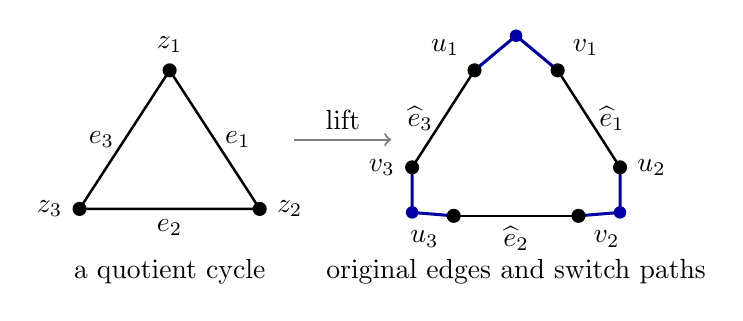
\begin{tikzpicture}[x=0.88cm,y=0.88cm,
  original/.style={line width=0.9pt},
  route/.style={line width=1.1pt,blue!65!black},
  vertex/.style={circle,fill=black,inner sep=1.8pt},
  inside/.style={circle,fill=blue!65!black,inner sep=1.6pt}]
\coordinate (z1) at (0,1.8);
\coordinate (z2) at (1.3,-0.2);
\coordinate (z3) at (-1.3,-0.2);
\draw[original] (z1)--node[right] {$e_1$}(z2)--node[below] {$e_2$}(z3)--node[left] {$e_3$}(z1);
\node[vertex,label=above:$z_1$] at (z1) {};
\node[vertex,label=right:$z_2$] at (z2) {};
\node[vertex,label=left:$z_3$] at (z3) {};
\node at (0,-1.1) {a quotient cycle};
\draw[->,gray,thick] (1.8,0.8)--(3.2,0.8);
\node[above] at (2.5,0.8) {lift};
\coordinate (u1) at (4.4,1.8);
\coordinate (v1) at (5.6,1.8);
\coordinate (u2) at (6.5,0.4);
\coordinate (v2) at (5.9,-0.3);
\coordinate (u3) at (4.1,-0.3);
\coordinate (v3) at (3.5,0.4);
\draw[original] (v1)--node[right] {$\widehat e_1$}(u2);
\draw[original] (v2)--node[below] {$\widehat e_2$}(u3);
\draw[original] (v3)--node[left] {$\widehat e_3$}(u1);
\draw[route] (u1)--(5,2.3)--(v1);
\draw[route] (u2)--(6.5,-0.25)--(v2);
\draw[route] (u3)--(3.5,-0.25)--(v3);
\node[inside] at (5,2.3) {};
\node[inside] at (6.5,-0.25) {};
\node[inside] at (3.5,-0.25) {};
\node[vertex,label=above left:$u_1$] at (u1) {};
\node[vertex,label=above right:$v_1$] at (v1) {};
\node[vertex,label=right:$u_2$] at (u2) {};
\node[vertex,label=below right:$v_2$] at (v2) {};
\node[vertex,label=below left:$u_3$] at (u3) {};
\node[vertex,label=left:$v_3$] at (v3) {};
\node at (5,-1.1) {original edges and switch paths};
\end{tikzpicture}
\caption{Lifting a quotient cycle, schematically. The fiber at \(z_j\)
contains \(u_j,v_j\); when they differ, a reserved path (blue) joins
them. The black edges are the unique original representatives of the
quotient edges. Every path interior avoids all black-edge endpoints,
and the interiors are pairwise disjoint for this cycle. Each blue
path is drawn with one internal vertex only for illustration; its
actual length may differ. A visit with \(u_j=v_j\) requires no path.}
\label{fig:cycle-lifting}
\end{figure}



\paragraph{The load bound over all batches.}
Fix one piece $R$.  Gather every demand for $P_R$ from all batches and
both constructions.  Each endpoint is in an active set, hence has
degree at most $a$ in the one graph $F(Y)$.  To bound its total demand
load, associate each occurrence of an endpoint $x$ with an incident
edge of $F(Y)$ as follows:
\begin{itemize}
 \item For the demand closing a remnant $L$, use the terminal edge of
       $L$ at $x$.
 \item At a switch $u_j\ne v_j$, associate the occurrence of $u_j$
       with $\widehat e_{j-1}$ and that of $v_j$ with $\widehat e_j$.
\end{itemize}
At a fixed vertex these associated incident edges are distinct.  For
the first construction this follows from the edge-disjoint path
partition and from the disjointness of the designated edge sets.
For the second construction a quotient edge belongs to exactly one
part, has exactly one original representative, and its incidence at a
given original vertex can be used only at the unique visit to its
quotient fiber in that cycle.  The cycles are simple, and a switch uses
different original vertices for its two incidences.  The two constructions
use disjoint edges because all designated edges were removed before
folding.  Finally, edges from different batches are distinct by
hypothesis, regardless of overlap of their vertex sets or differences
in their pairings.  This proves the injection into incident edges of
$F(Y)$ and hence
\begin{equation}\label{eq:batch-global-load}
 \text{number of demand-end occurrences at }x
 \le d_{F(Y)}(x)\le a.
\end{equation}
Vertices that are never endpoints have load zero.

\paragraph{Supplying all the connections.}
A team from a cycle $C$ has at most $s\le q_W\le B_0$ demands, and
$\abs{Z_C}\le2s\le2B_0$.  A heavy-neighbor remnant has at most
$\abs W\le B_0$ vertices; its team has size one.  Thus in
\Cref{lem:routing} we may use
\[
 r=r_R,\qquad h=\sigma/4,\qquad
 k=a,\qquad b=B_0,\qquad z=2B_0.
\]
With that lemma's definitions of $g$ and $\ell$, the range
$\sigma\le r_R\le D^{1.02}$ gives, uniformly in $R$,
\[
 \ell=O(D^{0.12}\log^2 D),
 \qquad
 \ell^2(a+B_0)+2B_0
       =O(D^{0.54}\log^4 D)=o(D^{0.90}).
\]
For all sufficiently large $D$ this is at most $\sigma/256=h/64$,
which is exactly enough for \eqref{eq:routing-condition}.  Apply the
routing lemma once to this full collection in $P_R$; if the collection
is empty, use no edges.  The paths supplied are pairwise edge-disjoint
over all teams and all batches for this $R$, and their internal vertex
sets are pairwise disjoint within each team.  Do this for every piece
$R$.  The constants are absolute, and do not depend on the number of
batches or demands.

\paragraph{Simplicity of the completed cycles.}
For a heavy-neighbor remnant $L$, its supplied path is simple and has
distinct endpoints equal to those of $L$.  Its internal vertices avoid
$V(L)$: the forbidden set contains $V(L)\cap V(R)$, and all supplied
path vertices lie in $V(R)$.  The union
is therefore a simple cycle.  It has at least two remnant edges and at
least one supplying edge, so its length is at least three.

For a quotient cycle $C$, the fibers of $z_1,\ldots,z_s$ are mutually
disjoint.  At a visit with $u_j=v_j$, its original representative edges
use one vertex.  At a switch, they use the two different vertices of
that fiber and the supplied simple path joins them.  Thus before
adding path interiors, the vertices at different visits are distinct.
Every supplying path interior avoids $Z_C$, which includes all these
original vertices.  Two supplying paths for this cycle in the same
router have disjoint interiors by their common team; paths in different
routers lie in the disjoint vertex sets of different pieces $R$.
Consequently interiors of any two switches are disjoint, and none
contains an endpoint of another switch or any other original vertex
used by the cycle.  Traversing the representatives and these connections
in cyclic order therefore visits no vertex twice, except the start
when closing the cycle.

An unused twin deserves explicit mention.  If a visited fiber is a pair
but $u_j=v_j$, its other vertex need not belong to $Z_C$ and may occur
inside a supplying path.  It is absent from all original representative
edges of this cycle, since those edges use distinct fibers.  If it is
used internally, no second supplying path of this cycle can use it:
the team condition excludes this in its router, and the other routers
have disjoint vertex sets.  This therefore creates no repeated vertex.
The same reasoning covers vertices in fibers not visited by the cycle.

The resulting cycle contains its $s$ distinct original representative
edges and possibly additional edges, so its length is at least
$s\ge3$.  A quotient cycle with no switches is already a simple cycle
of original edges.  Each quotient part thus yields exactly one permitted
part.

\paragraph{Edge accounting and cost.}
For each batch, its original edges have exactly four destinations:
\begin{enumerate}
 \item designated edges trimmed from paths are single-edge parts;
 \item designated edges in positive-length remnants occur in their
       closed cycles;
 \item folding error edges are single-edge parts, taken before
       identification;
 \item retained edges have unique representatives in $Q_W$ and occur
       once in the restored quotient parts.
\end{enumerate}
These classes partition $E(J_W)$.  Empty remnants leave no unaccounted
edge, and the deletion rule for parallel classes retains exactly one
representative for each quotient edge.  Since the $J_W$ have disjoint
edge sets, every edge of $F$ occurs once in this list over all batches.

Let $U_R$ be the set of edges used by all supplying paths in $P_R$.
Each is used once by the routing lemma.  These edges are disjoint from
$E(F)$ by hypothesis, and different routers have disjoint edge sets.
Thus all completed parts form an edge partition of the edge set in the
statement.  The heavy-neighbor work contributes at most $6\Sigma_Y$
parts, folding errors at most $2\Sigma_Y$, and the quotient partitions
contribute exactly $\sum_W t_W$.  Adding a supplying path changes no
part count.  This proves \eqref{eq:batch-parts}.

No edge of $T_R$ was used: $U_R\subseteq E(P_R)$ and $E(P_R)$ is
disjoint from $E(T_R)$.  Therefore $R'=R-U_R$ contains the entire
spanning graph $T_R$ on its original vertex set.  The edges of $R'$
are precisely the edges of this assigned piece not already used in a
completed part.  This proves both the remaining expansion assertion
and the final edge partition.
\end{proof}

\section{The induction}\label{sec:induction}

The preceding lemmas will be applied on a succession of scales. We
first select a prefix whose total piece order is controlled by one
of its layers. A fixed window beyond that layer makes the surviving
edges suitable for batching and folding.

Fix the absolute parameters
\begin{equation}\label{eq:induction-parameters}
 \theta=0.95,\qquad K=200,\qquad
 P_0=4(K+1),\qquad \eta=\frac1{100P_0}.
\end{equation}
In particular,
\begin{equation}\label{eq:scale-window}
 1.02\theta^K<0.001,\qquad \theta^{K+1}<0.001,
\end{equation}
since \(\theta^K\le e^{-10}\).

\begin{lemma}[Selection of a prefix]\label{lem:prefix-choice}
Let \((S_j)_{j\ge0}\) be a nonnegative, finitely supported sequence
which is not identically zero. There is an index \(i\) with
\(S_i>0\) such that
\begin{equation}\label{eq:prefix-charge}
 \sum_{j=0}^{i+K}S_j\le P_0S_i.
\end{equation}
\end{lemma}

\begin{proof}
Start at the first positive term and maintain
\(\sum_{j=0}^iS_j\le2(K+1)S_i\). If
\eqref{eq:prefix-charge} fails, the sum of the next \(K\) terms
is greater than \(2(K+1)S_i\). Their largest value \(M\) is
therefore greater than \(2S_i\). Move to an index \(i'\) in
that window with \(S_{i'}=M\). Then
\[
 \sum_{j=0}^{i'}S_j
 \le 2(K+1)S_i+KM
 <(2K+1)M\le2(K+1)S_{i'}.
\]
The invariant persists. Each move increases the index and lands
at a positive term. Finite support therefore forces the procedure
to stop, at which point \eqref{eq:prefix-charge} holds.
\end{proof}

For real \(x\ge1\), define the nondecreasing function
\begin{equation}\label{eq:induction-potential}
 \phi(1)=\frac12,\qquad
 \phi(x)=\max\left\{\frac12,
                1-\frac1{\sqrt{\log x}}\right\}
 \quad(x>1).
\end{equation}
The small improvement over a linear bound will absorb the overlap
introduced when boxes are split.

\begin{proposition}\label{prop:induction-bound}
There is an absolute constant \(C\) such that every finite simple
graph on \(n\ge1\) vertices has an edge partition into at most
\(C\phi(n)n\) simple cycles and single edges.
\end{proposition}

\begin{proof}
We use strong induction on \(n\). The lower scale cutoff \(D_*\)
is an absolute constant, chosen to satisfy the uniform requirements
below. Only after fixing it will we choose \(C\). All auxiliary
constants introduced before that final choice are independent of
\(C\) and remain valid if the cutoff is increased.

Edgeless graphs have the empty partition. For \(1\le n<D_*\),
using every edge singly proves the assertion when \(C\ge D_*\),
since \(\phi(n)\ge1/2\). Now let \(n\ge D_*\), assume the
assertion for every smaller positive order, and put
\[
 D_j=n^{\theta^j},\qquad
 m=\min\{j\ge0:D_j<D_*\}.
\]
Take \(D_*>2\). Then \(m\) is finite and positive, and the
scales \(D_0,\ldots,D_{m-1}\) all satisfy the cutoff.

\paragraph{Prospective layers.}
Starting with the given graph \(G\), perform both operations of
\Cref{lem:scale-split} at each successive scale
\(D_0,\ldots,D_{m-1}\). The inputs at stage \(j\) have average
degree at most \(D_j\): this holds initially because
\(\overline d(G)\le n-1<D_0\), and the residual graph in each
new box has average degree at most
\(D_j^{0.95}=D_{j+1}\).

Let \(\mathcal Y_j\) be the indexed family of level-\(j\)
boxes and \(\mathcal R_j\) the indexed family of pieces removed
inside them. The residual graph passed to the next stage retains
the entire vertex set of its box, including isolated vertices.
Every box has a unique indexed parent, and its vertex set is
contained in its parent's vertex set. Descendants of any box
cover that box's vertex set. Distinct indices are retained even
when their vertex sets overlap or coincide.

These operations define prospective layers: we will subsequently
keep only a prefix of them. At the end of every prefix, the long
cycles removed so far, the pieces removed so far, and the remaining
input graphs partition \(E(G)\). In particular, discarding the
prospective operations beyond a chosen prefix means retaining
their input graphs, with all their assigned edges, at that
prefix's boundary.

Write
\[
 N_{-1}=n,\qquad N_j=\sum_{Y\in\mathcal Y_j}|Y|,
 \qquad S_j=\sum_{R\in\mathcal R_j}|V(R)|,
\]
and set \(S_j=0\) for \(j\ge m\). Increase the absolute
constant \(C_0\) in \Cref{lem:scale-split} if necessary so that
\(C_0\ge1\), and put \(C_2=40C_0\). For \(0\le j<m\),
\[
 \sum_{l=0}^j\frac1{\log D_l}
 =\frac1{\log D_j}\sum_{t=0}^j\theta^t
 \le\frac{20}{\log D_j}.
\]
Provided \(\log D_*\ge C_2\), the product of the order
increases is consequently bounded by
\begin{equation}\label{eq:layer-order}
 n\le N_j
 \le n\prod_{l=0}^j\left(1+\frac{C_0}{\log D_l}\right)
 \le n\left(1+\frac{C_2}{\log D_j}\right)
 \le2n.
\end{equation}
Here we used \(1+x\le e^x\) and \(e^x\le1+2x\) for
\(0\le x\le1/2\). The lower bound follows from preservation
of the vertex cover at every split. The same product calculation,
using the relevant subproduct, shows that the orders of all
level-\(j\) descendants of a box of order \(y\) sum to at most
\((1+C_2/\log D_j)y\). Their union still covers its full
vertex set.

We also require \(D^{-0.01}\le1/\log D\) for every
\(D\ge D_*\). If \(\mathcal L_j\) is the family of long
cycles removed through level \(j\), then
\begin{equation}\label{eq:prefix-cycle-cost}
 |\mathcal L_j|
 \le\sum_{l=0}^j\frac{N_{l-1}}{2D_l^{0.01}}
 \le n\sum_{l=0}^j\frac1{\log D_l}
 \le\frac{20n}{\log D_j}.
\end{equation}
These bounds have no dependence on the number of layers.
Piece disjointness within each box gives
\(S_j\le N_j\le2n\).

\paragraph{Terminal cases.}
If every \(S_j\) vanishes, keep all prospective stages. Use the
long cycles and take the remaining edges singly. The remaining
graphs, on the level-\((m-1)\) boxes, have average degree at most
\(D_m<D_*\), so their total number of edges is at most
\(N_{m-1}D_m/2<D_*n\). By
\eqref{eq:prefix-cycle-cost}, the total cost is at most
\((20+D_*)n\).

Otherwise choose \(i\) by \Cref{lem:prefix-choice}. If
\(i+K\ge m-1\), again keep every stage. Retain all long cycles as
completed parts and take every edge of the final boundary graphs
singly, at cost at most \((20+D_*)n\) as above. The zero extension of
\((S_j)\) ensures that
\(\sum_{j=0}^{m-1}S_j\le P_0S_i\). Apply
\Cref{lem:small-residue} to each piece at its own scale, with
\(c=1\) and the fixed \(\eta\). This completes at most
\(9P_0S_i\) parts and leaves graphs of total order at most
\[
 \eta P_0S_i=\frac{S_i}{100}\le\frac n{50}<\frac n4.
\]
Each individual residual graph has order at most \(\eta r<n\),
where \(r\) is the order of its parent piece: the piece's
vertex set is a subset of \(V(G)\), so \(r\le n\), and
\(\eta<1\). Apply the induction hypothesis to each nonempty
residual graph; their total additional cost is at most \(Cn/4\),
using \(\phi\le1\).

Both terminal cases are therefore covered by the bound
\[
 T(D_*)n+\frac{Cn}{4},\qquad
 T(D_*)=20+D_*+18P_0.
\]
For \(C\ge4T(D_*)\), this is at most
\(Cn/2\le C\phi(n)n\). This choice also covers the base cases.

\paragraph{A prefix with a scale gap.}
It remains to consider \(i+K<m-1\). Keep the stages through
\(t=i+K\), and put
\begin{equation}\label{eq:batch-parameters}
 \begin{gathered}
 D=D_i,\qquad w=\log D,\qquad H=C_2\theta^{-K},\\
 B_0=D^{0.30},\qquad a=D^{0.01},\qquad
 L_0=D^{0.03},\qquad \sigma=D^{0.90}.
 \end{gathered}
\end{equation}
Since \(\log D_t=\theta^K w\),
\eqref{eq:layer-order} and \eqref{eq:prefix-cycle-cost} imply
\begin{equation}\label{eq:gap-global-bounds}
 N_t\le(1+H/w)n,\qquad |\mathcal L_t|\le Hn/w.
\end{equation}
The latter uses \(C_2\ge40>20\).

Fix a level-\(i\) box \(Y\), of order \(y\le D^{1.02}\).
Let \(T_Y\) be the sum of the orders of its level-\(t\)
descendants. Each such descendant carries its remaining graph
after stage \(t\); it has order at most
\(D^{1.02\theta^K}<D^{0.001}\) and that graph has average
degree at most \(D^{\theta^{K+1}}\). Moreover,
\begin{equation}\label{eq:descendant-order}
 y\le T_Y\le(1+H/w)y\le2y.
\end{equation}
For the last inequality, note that
\(H/w=C_2/\log D_t\le1\).

Let \(F(Y)\) be the graph on \(Y\) whose edges are exactly
the remaining edges in these descendants. Their assigned edge
sets are disjoint, so \(F(Y)\) is simple and
\begin{equation}\label{eq:descendant-degree}
 2|E(F(Y))|\le T_YD^{\theta^{K+1}}
 \le2yD^{\theta^{K+1}}.
\end{equation}

Each descendant has fewer than \(L_0\) vertices, so we first group
descendants to make larger folding sets possible. The number of
batches will bound the loss when an intersection of a batch with a
selected piece contains fewer than \(L_0\) vertices of degree at
most \(a\) in \(F(Y)\). The batch order cap \(B_0\) keeps quotient
cycles within the routing team bound.

Partition the indexed descendants into batches whose sums of
orders are at most \(B_0\). This can be done with at most
\(1+4y/B_0\) batches: require the cutoff to ensure
\(D^{0.001}\le B_0/2\), fill a batch until the next descendant
would exceed \(B_0\), and then start a new one. Every batch
except possibly the last has order sum greater than \(B_0/2\),
so their number is at most \(1+2T_Y/B_0\).

For each batch let \(W\) be the union of its vertex sets, and
let \(J_W\) contain exactly its remaining assigned edges. The
batch index is retained in this notation. Denote the family by
\(\mathcal W(Y)\). Thus the \(J_W\) partition \(E(F(Y))\),
the sets \(W\) cover \(Y\), and
\begin{equation}\label{eq:batch-orders}
 |W|\le B_0,\qquad
 \sum_{W\in\mathcal W(Y)}|W|\le T_Y,\qquad
 \sum_{Y\in\mathcal Y_i}\sum_{W\in\mathcal W(Y)}|W|
 \le N_t.
\end{equation}
The order sums used in forming batches include all descendant
multiplicities; passing to a union within a batch can only
decrease them.

Since each level-\(t\) box has a unique indexed level-\(i\)
ancestor, the batch edge sets over all \(Y\) partition the boundary
remainder. Thus, at the boundary of the committed prefix, the
assigned edge sets give the disjoint union
\begin{equation}\label{eq:global-edge-ledger}
 E(G)=
 \mathop{\dot\bigcup}_{L\in\mathcal L_t}E(L)
 \;\dot\cup\;
 \mathop{\dot\bigcup}_{j=0}^{t}\ 
             \mathop{\dot\bigcup}_{R\in\mathcal R_j}E(R)
 \;\dot\cup\;
 \mathop{\dot\bigcup}_{Y\in\mathcal Y_i}\ 
             \mathop{\dot\bigcup}_{W\in\mathcal W(Y)}E(J_W).
\end{equation}

\paragraph{Active sets and multiplicities.}
Call a vertex of \(Y\) good if its degree in \(F(Y)\) is at
most \(a\). By \eqref{eq:descendant-degree} and
\eqref{eq:scale-window}, the number of other vertices is at most
\[
 2yD^{\theta^{K+1}-0.01}\le2yD^{-0.009}\le y/w,
\]
where the final inequality is another uniform large-scale
requirement. For each \(W\in\mathcal W(Y)\) and each
level-\(i\) piece \(R\) belonging to \(Y\), consider all
good vertices of \(W\cap V(R)\). If their number is at least
\(L_0\), retain this set as \(X_{W,R}\) and call it active;
otherwise skip it. Active sets in a fixed batch are disjoint,
because the pieces in \(Y\) have disjoint vertex sets.

There are at most \(y/\sigma\) such pieces. Consequently the
total size of all skipped sets in \(Y\), counting occurrences
in different batches separately, is at most
\begin{align}
 L_0(1+4y/B_0)y/\sigma
 &\le y\bigl(D^{-0.87}+4D^{-0.15}\bigr)
 \le y/w.\label{eq:skipped-occurrences}
\end{align}
Here the exponent \(-0.15\) uses \(y\le D^{1.02}\), and the
last inequality is imposed for all scales above the cutoff.

Let \(s(Y)\) be the sum of the orders of the level-\(i\)
pieces in \(Y\), and define
\[
 \Sigma_Y=\sum_{\substack{W\in\mathcal W(Y),\ R\text{ in }Y\\
                         X_{W,R}\text{ active}}}|X_{W,R}|,
 \qquad \Sigma=\sum_{Y\in\mathcal Y_i}\Sigma_Y.
\]
Every good piece vertex occurs in at least one batch, since the
batches cover \(Y\). Choose one such occurrence per vertex.
At most \(y/w\) piece vertices are not good, and at most
\(y/w\) of the chosen occurrences can lie in skipped sets by
\eqref{eq:skipped-occurrences}. Hence
\(\Sigma_Y\ge s(Y)-2y/w\).

For the upper bound, let \(u_Y(v)\ge1\) be the number of
batches in \(Y\) containing \(v\). Then
\[
 \sum_{v\in Y}\bigl(u_Y(v)-1\bigr)
 =\sum_{W\in\mathcal W(Y)}|W|-y.
\]
Since the pieces in \(Y\) are vertex-disjoint, their excess
occurrences are bounded by this full excess. Thus
\(\Sigma_Y\le s(Y)+\sum_W|W|-y\). Summing the two bounds,
using \(N_i\le2n\), \(N_i\ge n\), and
\eqref{eq:gap-global-bounds}--\eqref{eq:batch-orders}, gives
\begin{equation}\label{eq:active-order}
 S_i-\frac{4n}{w}\le\Sigma
 \le S_i+N_t-N_i\le S_i+\frac{Hn}{w}.
\end{equation}
This counts a nongood vertex only once per indexed box in the
lower bound; no bound on its number of batch occurrences is
needed. Overlaps between different boxes are already included
in both \(S_i\) and \(N_i\).

\paragraph{Resolving the batches and the pieces.}
In every level-\(i\) piece \(R\), apply
\Cref{lem:edge-split} with two classes to partition its assigned
edges into spanning graphs \(P_R\) and \(T_R\), each with
cut expansion at least \(\sigma/4\). Reserve \(P_R\) as a
router and leave \(T_R\) untouched during the batch work.

All hypotheses of \Cref{lem:batch-resolution} now hold in each
\(Y\). The \(J_W\) have order at most \(B_0\) and disjoint
assigned edges; their union is \(F(Y)\). The pieces have
orders between \(\sigma\) and \(D^{1.02}\), disjoint vertex
sets within \(Y\), and edges disjoint from \(F(Y)\).
Every vertex of an active \(X_{W,R}\) has
degree at most \(a\) in the whole \(F(Y)\), and its active
set has order at least \(L_0\). In particular the degree bound
is shared across all batches, as required by that lemma.

The lemma produces simple quotient graphs \(Q_W\), with orders
\begin{equation}\label{eq:individual-quotient-order}
 q_W=|W|-\sum_{R:X_{W,R}\text{ active}}
                       \floor{|X_{W,R}|/2}
 \le |W|-\frac13\sum_{R:X_{W,R}\text{ active}}|X_{W,R}|.
\end{equation}
Every batch has positive order and pair identifications leave
at least one vertex, so \(1\le q_W\le B_0\). Also
\(B_0=D^{0.30}\le n^{0.30}<n\). Apply the induction
hypothesis to these quotients, retaining isolated quotient
vertices in their order counts. The batch lemma lifts all the
resulting quotient parts simultaneously. In each \(Y\), the
additional number of completed parts is at most \(8\Sigma_Y\),
and the remaining graph on every \(R\) still contains \(T_R\).
In particular, lifting a quotient cycle produces one simple
cycle and has no additional part charge.

Apply \Cref{lem:small-residue}, with the fixed \(\eta\), to
the remaining graph of every level-\(i\) piece using \(c=1/4\).
Apply it to every other piece of the committed prefix at its
own scale using \(c=1\). The total number of parts supplied
by these applications is at most \(9P_0S_i\). If
\(\mathcal H\) is their family of residual graphs, then
\begin{equation}\label{eq:piece-residual-order}
 \sum_{H'\in\mathcal H}|V(H')|
 \le\eta\sum_{j=0}^tS_j\le\eta P_0S_i.
\end{equation}
Every nonempty member has order at most \(\eta r<n\), for
the same reason as in the terminal case. Induction applies to
all of them.

Within each \(Y\), \Cref{lem:batch-resolution} resolves exactly
the batch category in \eqref{eq:global-edge-ledger} together
with the router edges it consumes.
Every consumed router edge comes from exactly one level-\(i\)
piece and is used once. The piece lemmas are applied only after
those edges have been removed, and partition all remaining
piece edges into completed parts and the members of
\(\mathcal H\). Distinct indexed boxes have disjoint assigned
edge sets even when their vertex sets overlap. Thus the only
unresolved original edges after lifting the quotient partitions
are precisely the assigned edges of \(\mathcal H\), each
appearing once. Recursively partitioning them completes an edge
partition of \(G\).

\paragraph{Order savings and the final estimate.}
Define the absolute constants
\[
 A_1=H+\frac43,\qquad
 A_2=\max\{9P_0+8,\,9H\}.
\]
By \eqref{eq:individual-quotient-order},
\eqref{eq:batch-orders}, and \eqref{eq:active-order},
\begin{equation}\label{eq:total-quotient-order}
 \sum_{Y,W}q_W\le N_t-\frac{\Sigma}{3}
 \le n-\frac{S_i}{3}+\frac{A_1n}{w}.
\end{equation}
The parts completed apart from the quotient partitions and
the recursive work on \(\mathcal H\) number at most
\begin{align}
 |\mathcal L_t|+8\Sigma+9P_0S_i
 &\le (9P_0+8)S_i+9Hn/w\notag\\
 &\le A_2(S_i+n/w).\label{eq:nonrecursive-cost}
\end{align}
Monotonicity of \(\phi\), \(q_W\le B_0\), and
\eqref{eq:piece-residual-order} therefore bound the complete
partition size by
\begin{equation}\label{eq:inductive-cost}
 A_2(S_i+n/w)+C\eta P_0S_i
 +C\phi(B_0)\left(n-\frac{S_i}{3}+\frac{A_1n}{w}\right).
\end{equation}
The coefficient of \(S_i\) in this expression is at most
\[
 A_2+\frac C{100}-\frac C6
 =A_2-\frac{47C}{300}\le0
 \qquad\text{if }C\ge7A_2.
\]
It remains to pay for the order-overlap term. Set
\(\delta=1/\sqrt{0.30}-1>0\). For \(w\ge40/3\), both
\(\phi(n)\) and \(\phi(B_0)\) take their nonconstant
values, and \(\log n\ge w\) gives
\begin{equation}\label{eq:potential-gain}
 \phi(n)-\phi(B_0)
 =\frac1{\sqrt{0.30w}}-\frac1{\sqrt{\log n}}
 \ge\frac{\delta}{\sqrt w}.
\end{equation}
For \(C\ge7A_2\), the remaining overhead in
\eqref{eq:inductive-cost}, beyond \(C\phi(B_0)n\), is at
most \(C(A_1+1)n/w\). It is absorbed by
\eqref{eq:potential-gain} whenever
\begin{equation}\label{eq:cutoff-absorption}
 \log D_*\ge\left(\frac{A_1+1}{\delta}\right)^2.
\end{equation}
No choice made here requires the total quotient order in
\eqref{eq:total-quotient-order} to be at most \(n\); the
potential gain pays for its possible excess.

We finally specify the order of constant choices. The parameters
in \eqref{eq:induction-parameters}, the scale-split constant
\(C_0\ge1\), and hence \(C_2,H,A_1,A_2,\delta\), are
already absolute and fixed. Choose \(D_*\) large enough for
\Cref{lem:scale-split,lem:batch-resolution}, for
\Cref{lem:edge-split} with two classes at expansion
\(D^{0.90}\), and for \Cref{lem:small-residue} with the
fixed \(\eta\) and \(c\in\{1,1/4\}\). Also impose
\(\log D_*\ge\max\{C_2,40/3\}\),
\eqref{eq:cutoff-absorption}, and, for every \(D\ge D_*\),
\[
 \begin{gathered}
 D^{-0.01}\le\frac1{\log D},\qquad
 D^{0.001}\le\tfrac12D^{0.30},\\
 2D^{-0.009}\le\frac1{\log D},\qquad
 D^{-0.87}+4D^{-0.15}\le\frac1{\log D}.
 \end{gathered}
\]
These are uniform eventual inequalities between fixed powers
and logarithms. Such a cutoff exists independently of \(C\).
After fixing it, choose
\[
 C\ge\max\{7A_2,\,4T(D_*)\}.
\]
The base and terminal cases then hold, and
\eqref{eq:inductive-cost}--\eqref{eq:potential-gain} give at
most \(C\phi(n)n\) parts in the remaining case. This closes
the strong induction.
\end{proof}

Since \(\phi(n)\le1\), \Cref{prop:induction-bound} proves
\Cref{thm:main} for positive order. The zero-vertex graph has
the empty partition, completing all cases.


\bibliographystyle{plain}
\bibliography{references}
\end{document}
